\documentclass[12pt,a4paper]{report}

% ============================================================
% PACKAGES
% ============================================================
\usepackage[margin=3cm,bindingoffset=0.5cm]{geometry}
\usepackage[utf8]{inputenc}
\usepackage[T1]{fontenc}
\usepackage[bahasa]{babel}
\usepackage{graphicx}
\usepackage{booktabs}
\usepackage{longtable}
\usepackage{array}
\usepackage{float}
\usepackage{xcolor}
\usepackage{hyperref}
\usepackage{caption}
\usepackage{fancyhdr}
\usepackage{titlesec}
\usepackage{amsmath}
\usepackage{enumitem}
\usepackage{setspace}
\onehalfspacing

\graphicspath{{evidence/}}

\hypersetup{
    colorlinks=true,
    linkcolor=black,
    urlcolor=blue,
    citecolor=black,
    pdftitle={Tesis - Prediksi Kondisi Kesehatan SIV TS27},
}

% --- Format Judul BAB gaya skripsi Indonesia ---
\titleformat{\chapter}[display]
  {\normalfont\bfseries\centering}{BAB \Roman{chapter}}{10pt}{\Large\bfseries}
\titlespacing*{\chapter}{0pt}{0pt}{30pt}

\pagestyle{fancy}
\fancyhf{}
\fancyhead[L]{\small Prediksi Kondisi Kesehatan SIV TS27 — TCN + MLP}
\fancyhead[R]{\small\thepage}
\renewcommand{\headrulewidth}{0.4pt}

\newcommand{\healthy}{\textcolor{teal}{\textbf{Healthy}}}
\newcommand{\warning}{\textcolor{orange!80!black}{\textbf{Warning}}}
\newcommand{\ok}{\textcolor{teal}{\checkmark}}
\newcommand{\bad}{\textcolor{red}{$\times$}}

\begin{document}

% ============================================================
% HALAMAN JUDUL
% ============================================================
\begin{titlepage}
\begin{center}
\vspace*{1cm}
{\large [NAMA UNIVERSITAS]}\\[0.3cm]
{\large FAKULTAS [NAMA FAKULTAS]}\\[0.3cm]
{\large PROGRAM STUDI [NAMA PROGRAM STUDI]}\\[2.5cm]

{\Large\bfseries PREDIKSI DINI KONDISI KESEHATAN\\
STATIC INVERTER (SIV) TS27 MENGGUNAKAN\\
PENDEKATAN DUA TAHAP TEMPORAL CONVOLUTIONAL\\
NETWORK (TCN) DAN MULTI-LAYER PERCEPTRON (MLP)}\\[0.5cm]

{\large [Judul dapat disesuaikan dengan ketentuan pembimbing/kampus]}\\[3cm]

{\large TESIS / SKRIPSI}\\[0.3cm]
{\normalsize Diajukan untuk memenuhi salah satu syarat memperoleh gelar\\
[Sarjana/Magister] [Nama Program Studi]}\\[3cm]

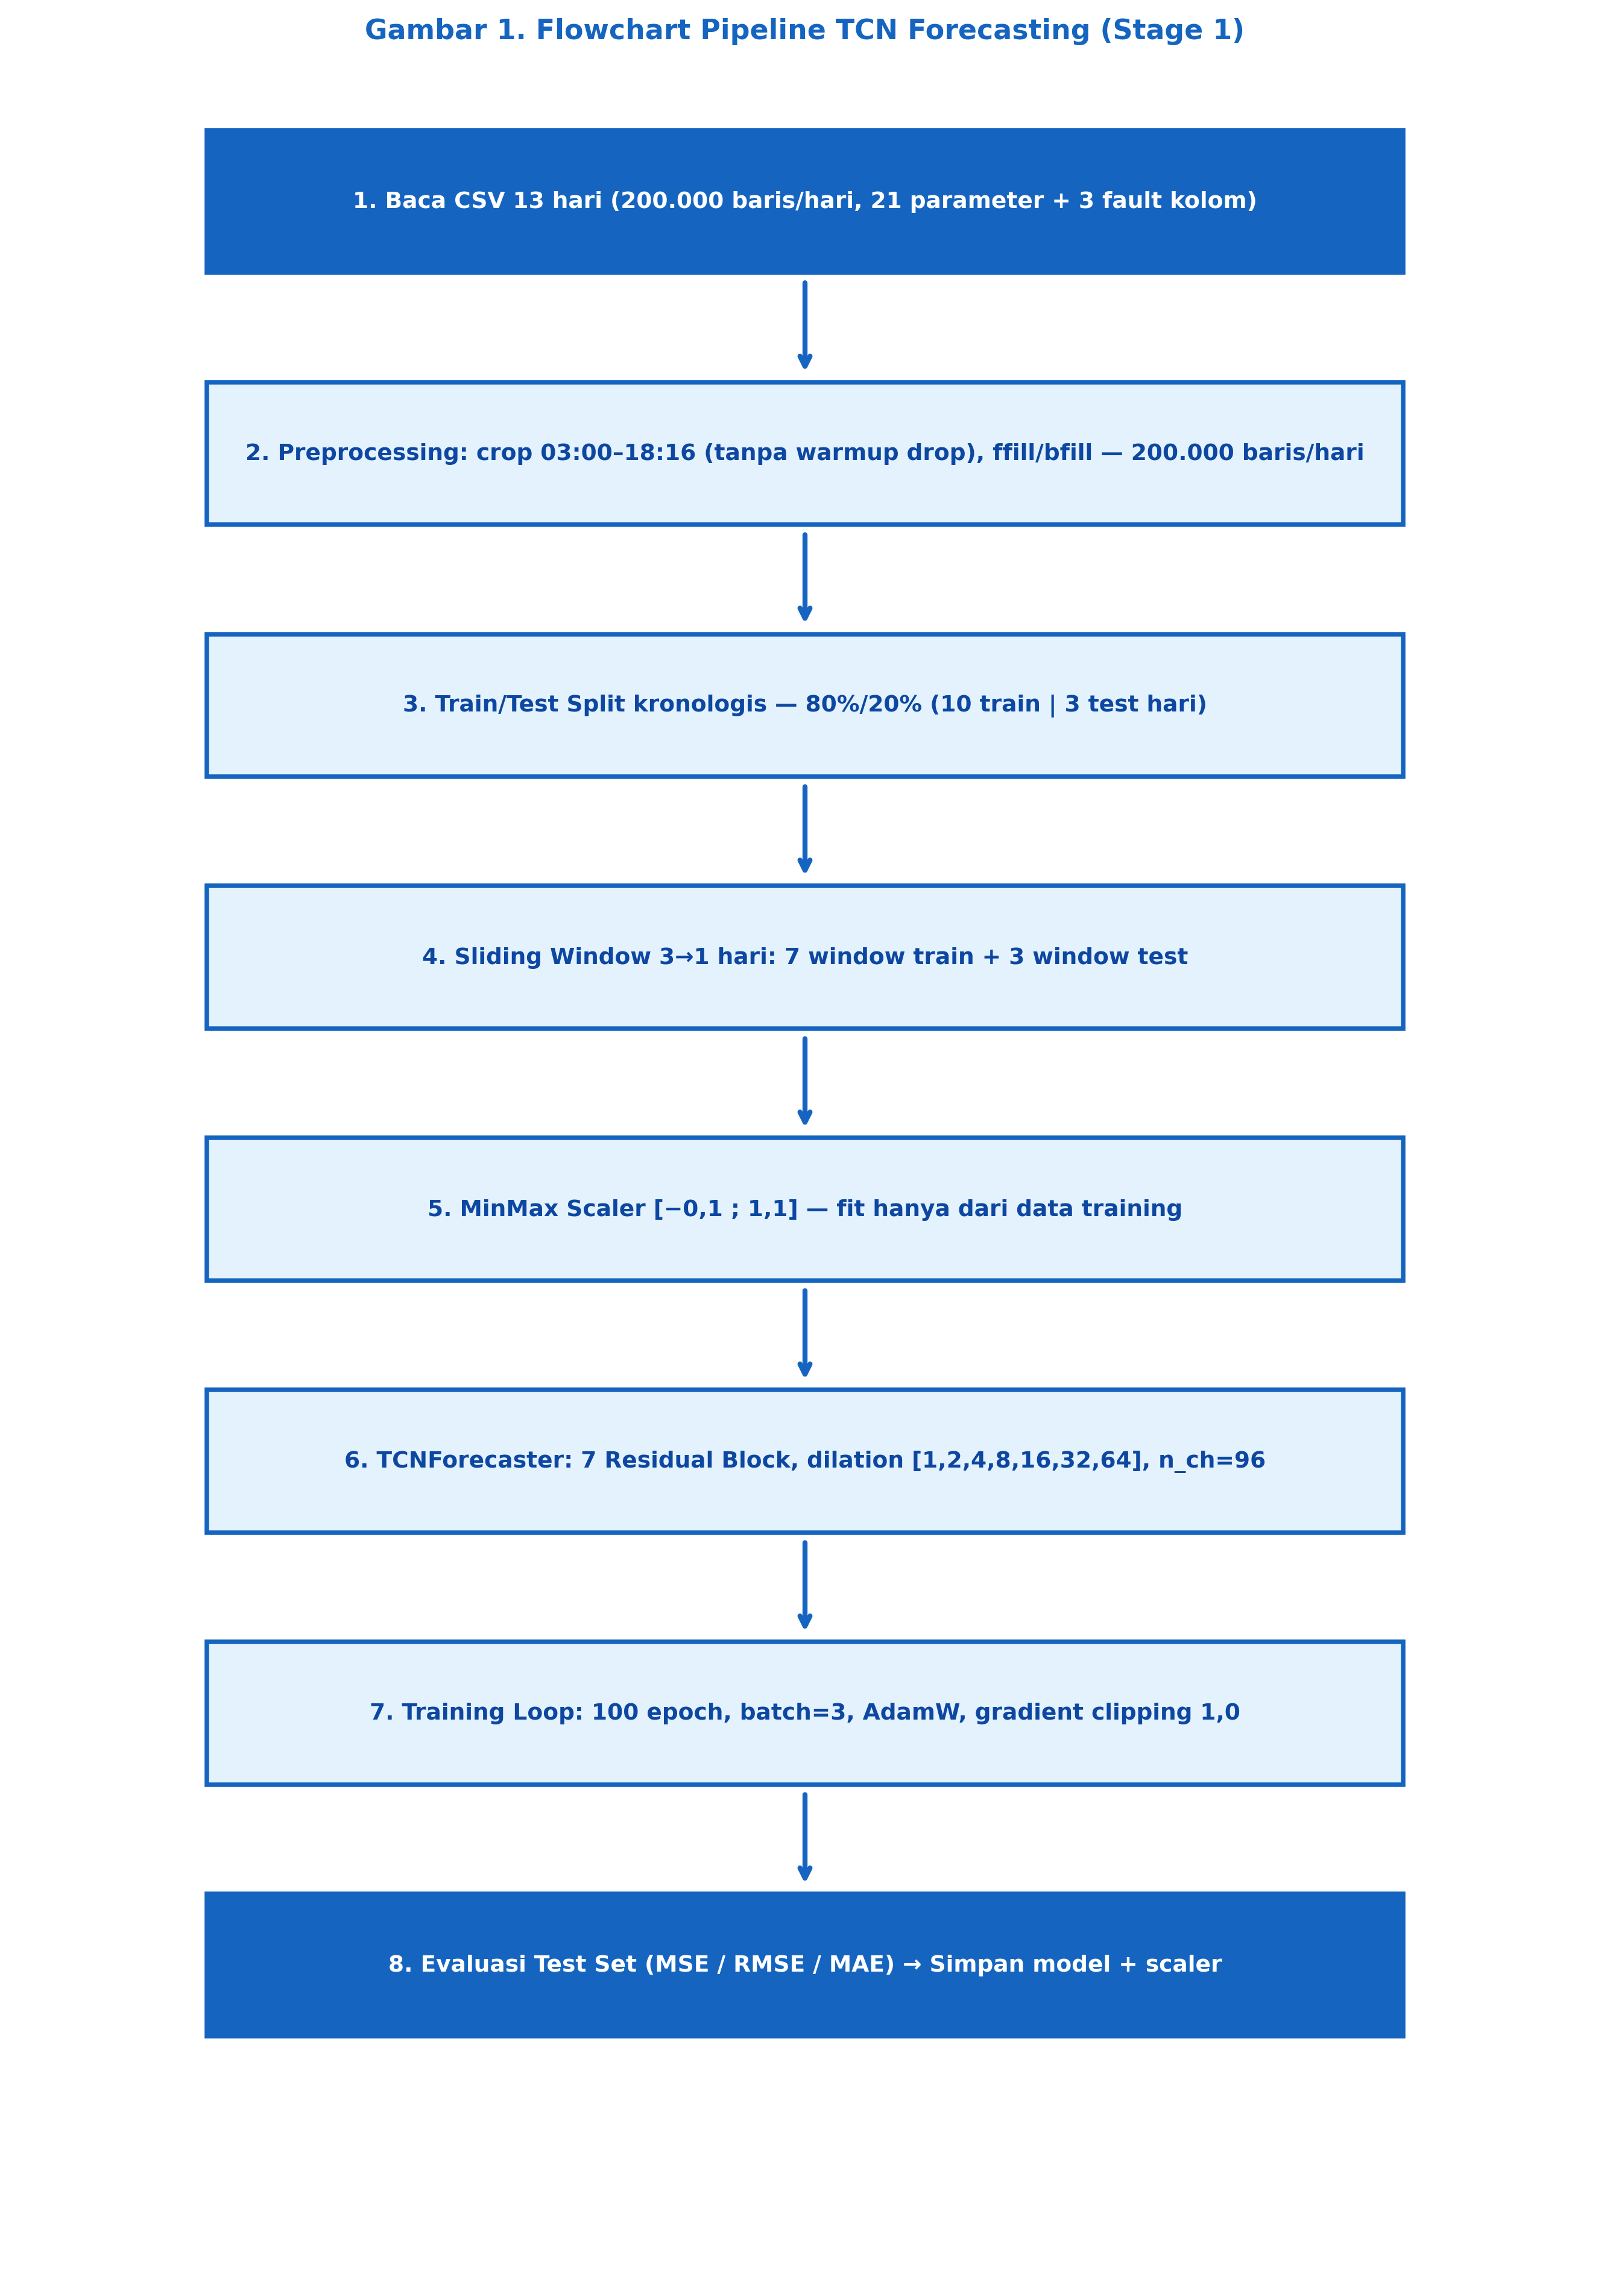
\includegraphics[width=3cm]{jurnal_flowchart_stage1.png}\\[0.3cm]
{\small\textit{(Ganti dengan logo institusi)}}\\[2cm]

\begin{tabular}{ll}
Disusun oleh: & [NAMA MAHASISWA] \\
NIM: & [NOMOR INDUK MAHASISWA] \\
Dosen Pembimbing: & [NAMA DOSEN PEMBIMBING] \\
\end{tabular}\\[2cm]

{\large [NAMA KOTA]}\\
{\large [TAHUN]}
\end{center}
\end{titlepage}

% ============================================================
% LEMBAR PENGESAHAN
% ============================================================
\chapter*{Lembar Pengesahan}
\addcontentsline{toc}{chapter}{Lembar Pengesahan}

\noindent Tesis/Skripsi berjudul \textbf{"Prediksi Dini Kondisi Kesehatan Static Inverter (SIV) TS27 Menggunakan Pendekatan Dua Tahap Temporal Convolutional Network (TCN) dan Multi-Layer Perceptron (MLP)"} yang disusun oleh:

\begin{center}
\begin{tabular}{ll}
Nama & : [NAMA MAHASISWA] \\
NIM  & : [NOMOR INDUK MAHASISWA] \\
Program Studi & : [NAMA PROGRAM STUDI] \\
\end{tabular}
\end{center}

\noindent telah dipertahankan di hadapan Tim Penguji pada tanggal [TANGGAL SIDANG] dan dinyatakan telah memenuhi syarat.

\vspace{2cm}
\noindent\textit{(Halaman ini perlu ditandatangani oleh dosen pembimbing dan penguji sesuai format institusi masing-masing.)}

% ============================================================
% PERNYATAAN KEASLIAN
% ============================================================
\chapter*{Pernyataan Keaslian}
\addcontentsline{toc}{chapter}{Pernyataan Keaslian}
\noindent Saya yang bertanda tangan di bawah ini menyatakan bahwa tesis/skripsi ini adalah hasil karya saya sendiri dan belum pernah diajukan untuk memperoleh gelar akademik di institusi mana pun. Seluruh sumber informasi yang dikutip telah dicantumkan sesuai kaidah penulisan ilmiah yang berlaku.

\vspace{2cm}
\noindent [Nama Kota], [Tanggal] \\[2cm]
\noindent [NAMA MAHASISWA] \\
NIM. [NOMOR INDUK MAHASISWA]

% ============================================================
% ABSTRAK
% ============================================================
\chapter*{Abstrak}
\addcontentsline{toc}{chapter}{Abstrak}

\noindent Static Inverter (SIV) merupakan komponen elektronik daya yang berfungsi mengonversi tegangan DC baterai menjadi tegangan AC untuk memasok kebutuhan daya bantu (\textit{auxiliary power}). Kegagalan pada unit SIV dapat menyebabkan gangguan operasional yang signifikan, sehingga diperlukan sistem deteksi dini (\textit{early warning system}) berbasis data historis sensor. Penelitian ini mengusulkan pendekatan dua tahap (\textit{two-stage pipeline}) menggunakan \textbf{Temporal Convolutional Network (TCN)} sebagai model \textit{forecasting} 21 parameter sensor untuk 1 hari ke depan berdasarkan 3 hari data sebelumnya, dilanjutkan dengan \textbf{Multi-Layer Perceptron (MLP) Classifier} yang mengklasifikasikan status kesehatan harian menjadi \textit{Healthy} atau \textit{Warning} berdasarkan 84 fitur statistik hasil \textit{forecast}. Dataset terdiri atas 37 hari data valid unit SIV TS27 (29 hari \textit{training}, 8 hari \textit{testing}), masing-masing berisi 200.000 baris pembacaan sensor per hari. Hasil pengujian menunjukkan model TCN mencapai MSE \textit{test} sebesar 0,0074 (RMSE 0,0863; MAE 0,0433) tanpa indikasi \textit{overfitting} signifikan. Sementara itu, model MLP Classifier mencapai akurasi \textit{training} 100\% namun akurasi \textit{testing} hanya 62,5\% dengan F1-\textit{score} 48,08\%, mengindikasikan \textit{overfitting} yang disebabkan oleh terbatasnya jumlah sampel berlabel (29 sampel \textit{training}, hanya 9 sampel kelas \textit{Warning}). Penelitian ini menyimpulkan bahwa pendekatan \textit{forecasting} berbasis TCN layak digunakan, namun tahap klasifikasi memerlukan penambahan data dan regularisasi lebih lanjut agar dapat digeneralisasi dengan baik.

\vspace{0.5cm}
\noindent\textbf{Kata kunci:} Static Inverter, Temporal Convolutional Network, Multi-Layer Perceptron, prediksi kesehatan, \textit{time series forecasting}, \textit{early warning system}.

\chapter*{Abstract}
\addcontentsline{toc}{chapter}{Abstract}
\noindent\textit{[Terjemahan Bahasa Inggris dari abstrak di atas — lengkapi sesuai kebutuhan institusi.]}

% ============================================================
% KATA PENGANTAR
% ============================================================
\chapter*{Kata Pengantar}
\addcontentsline{toc}{chapter}{Kata Pengantar}
\noindent [Tulis ucapan syukur, latar belakang penyusunan, dan ucapan terima kasih kepada dosen pembimbing, institusi, keluarga, dan pihak-pihak terkait di sini.]

% ============================================================
% DAFTAR ISI, GAMBAR, TABEL
% ============================================================
\tableofcontents
\listoffigures
\listoftables

\newpage

% ============================================================
\chapter{PENDAHULUAN}
% ============================================================

\section{Latar Belakang}
Static Inverter (SIV) adalah komponen elektronik daya yang berfungsi mengubah tegangan DC dari baterai menjadi tegangan AC untuk memasok kebutuhan daya bantu (\textit{auxiliary power}) pada sistem kelistrikan kendaraan maupun peralatan industri. Sebagai komponen kritis, kegagalan fungsi SIV dapat mengakibatkan gangguan operasional yang berdampak pada keandalan sistem secara keseluruhan. Pemeliharaan berbasis jadwal (\textit{scheduled maintenance}) yang umum diterapkan saat ini memiliki keterbatasan karena tidak mempertimbangkan kondisi aktual komponen, sehingga berpotensi menyebabkan kegagalan mendadak (\textit{unplanned failure}) atau pemeliharaan yang tidak efisien.

Perkembangan teknologi \textit{Internet of Things} (IoT) memungkinkan pengumpulan data sensor secara kontinu dari unit SIV, seperti suhu, arus, dan tegangan pada berbagai titik ukur. Data historis ini berpotensi dimanfaatkan untuk membangun model \textit{predictive maintenance} berbasis \textit{deep learning} yang mampu memprediksi kondisi kesehatan unit secara dini, sebelum kegagalan benar-benar terjadi.

Penelitian ini mengusulkan pendekatan dua tahap: (1) \textbf{Temporal Convolutional Network (TCN)} untuk melakukan \textit{forecasting} nilai parameter sensor di masa depan, dan (2) \textbf{Multi-Layer Perceptron (MLP)} untuk mengklasifikasikan status kesehatan (\textit{Healthy}/\textit{Warning}) berdasarkan hasil \textit{forecast} tersebut. Pendekatan ini dipilih karena TCN dikenal efektif menangkap pola temporal jangka panjang melalui \textit{dilated causal convolution}, sementara MLP mampu mempelajari relasi non-linear antar fitur statistik untuk tugas klasifikasi.

\section{Rumusan Masalah}
Berdasarkan latar belakang di atas, rumusan masalah penelitian ini adalah:
\begin{enumerate}
    \item Bagaimana performa model TCN dalam memprediksi nilai 21 parameter sensor SIV TS27 untuk 1 hari ke depan berdasarkan data 3 hari sebelumnya?
    \item Bagaimana performa model MLP Classifier dalam mengklasifikasikan status kesehatan (\textit{Healthy}/\textit{Warning}) berdasarkan fitur statistik hasil \textit{forecast} TCN?
    \item Apakah pendekatan dua tahap ini dapat digeneralisasi dengan baik pada data yang belum pernah dilihat model (data \textit{testing})?
\end{enumerate}

\section{Tujuan Penelitian}
\begin{enumerate}
    \item Membangun dan mengevaluasi model TCN untuk \textit{forecasting} parameter sensor SIV TS27.
    \item Membangun dan mengevaluasi model MLP Classifier untuk klasifikasi status kesehatan SIV TS27.
    \item Menganalisis kemampuan generalisasi kedua model melalui perbandingan metrik \textit{training} dan \textit{testing}.
\end{enumerate}

\section{Batasan Masalah}
\begin{enumerate}
    \item Data yang digunakan adalah data historis sensor unit SIV TS27 selama 37 hari, masing-masing 200.000 baris pembacaan per hari.
    \item Model \textit{forecasting} menggunakan arsitektur TCN dengan \textit{input window} 3 hari dan \textit{output horizon} 1 hari.
    \item Model klasifikasi menggunakan arsitektur MLP dengan input 84 fitur statistik (\textit{mean}, \textit{std}, \textit{min}, \textit{max} dari 21 parameter).
    \item Status kesehatan dibatasi pada dua kelas: \textit{Healthy} dan \textit{Warning}.
    \item Penelitian ini tidak membahas implementasi sistem \textit{real-time monitoring} secara penuh, melainkan berfokus pada pengembangan dan evaluasi model.
\end{enumerate}

\section{Manfaat Penelitian}
\begin{enumerate}
    \item \textbf{Manfaat Teoritis}: memberikan kontribusi referensi penerapan pendekatan dua tahap (\textit{forecasting} + klasifikasi) menggunakan TCN dan MLP pada domain \textit{predictive maintenance} peralatan elektronik daya.
    \item \textbf{Manfaat Praktis}: hasil penelitian dapat menjadi dasar pengembangan sistem \textit{early warning} untuk mendeteksi potensi gangguan SIV secara dini, sehingga dapat mengurangi risiko kegagalan mendadak dan mengoptimalkan jadwal pemeliharaan.
\end{enumerate}

\section{Sistematika Penulisan}
Tesis/skripsi ini disusun dalam lima bab. \textbf{BAB I} membahas latar belakang, rumusan masalah, tujuan, batasan, dan manfaat penelitian. \textbf{BAB II} membahas tinjauan pustaka meliputi teori \textit{time series forecasting}, TCN, MLP, dan metrik evaluasi. \textbf{BAB III} membahas metodologi penelitian meliputi dataset, \textit{preprocessing}, dan arsitektur model. \textbf{BAB IV} membahas hasil eksperimen dan pembahasan. \textbf{BAB V} membahas kesimpulan dan saran.

\newpage
% ============================================================
\chapter{TINJAUAN PUSTAKA}
% ============================================================

\section{Predictive Maintenance}
\textit{Predictive maintenance} adalah strategi pemeliharaan yang memanfaatkan data kondisi aktual peralatan untuk memprediksi kapan kegagalan berpotensi terjadi, sehingga tindakan pemeliharaan dapat dilakukan tepat waktu. Pendekatan ini berbeda dengan \textit{preventive maintenance} yang bersifat terjadwal tanpa mempertimbangkan kondisi riil komponen. Dalam konteks penelitian ini, \textit{predictive maintenance} diterapkan pada unit Static Inverter (SIV) berbasis data sensor time-series.

\section{Time Series Forecasting}
\textit{Time series forecasting} adalah proses memprediksi nilai masa depan berdasarkan pola data historis yang terurut menurut waktu. Pendekatan berbasis \textit{deep learning} seperti \textit{Recurrent Neural Network} (RNN), \textit{Long Short-Term Memory} (LSTM), dan \textit{Temporal Convolutional Network} (TCN) telah banyak digunakan karena kemampuannya menangkap pola temporal non-linear yang kompleks.

\section{Temporal Convolutional Network (TCN)}
TCN adalah arsitektur \textit{deep learning} berbasis \textit{convolutional neural network} yang dirancang khusus untuk data sekuensial. TCN menggunakan \textit{dilated causal convolution} untuk memperluas \textit{receptive field} secara eksponensial tanpa menambah jumlah parameter secara signifikan, serta \textit{residual connection} untuk menstabilkan proses training pada jaringan yang dalam. Dibandingkan RNN/LSTM, TCN memiliki keunggulan berupa komputasi paralel dan gradien yang lebih stabil karena tidak bergantung pada struktur rekursif.

Pada penelitian ini, arsitektur TCN yang digunakan terdiri atas 7 \textit{residual block} dengan faktor dilasi $[1, 2, 4, 8, 16, 32, 64]$, 96 \textit{hidden channel}, dan \textit{kernel size} 3 (detail lengkap pada Bab III).

\section{Multi-Layer Perceptron (MLP)}
MLP adalah arsitektur \textit{feedforward neural network} yang terdiri atas beberapa lapisan (\textit{layer}) neuron yang saling terhubung penuh (\textit{fully connected}). MLP umum digunakan untuk tugas klasifikasi berbasis fitur tabular. Pada penelitian ini, MLP digunakan untuk mengklasifikasikan status kesehatan SIV berdasarkan fitur statistik yang diringkas dari hasil \textit{forecasting} TCN.

\section{Normalisasi Data}
Normalisasi \textit{Min-Max Scaler} digunakan untuk menyamakan skala antar parameter sensor yang memiliki rentang nilai berbeda-beda, sehingga proses training model menjadi lebih stabil. Normalisasi dilakukan dengan formula:
\begin{equation}
    x' = \frac{x - x_{min}}{x_{max} - x_{min}} \times (b - a) + a
\end{equation}
dengan $a$ dan $b$ adalah batas bawah dan atas rentang target normalisasi.

\section{Metrik Evaluasi}
\subsection{Metrik Regresi (Forecasting)}
\begin{itemize}
    \item \textbf{Mean Squared Error (MSE)}: rata-rata kuadrat selisih antara nilai aktual dan prediksi.
    \item \textbf{Root Mean Squared Error (RMSE)}: akar dari MSE, memiliki satuan yang sama dengan data asli.
    \item \textbf{Mean Absolute Error (MAE)}: rata-rata nilai absolut selisih aktual dan prediksi.
    \item \textbf{Mean Absolute Percentage Error (MAPE)}: rata-rata persentase kesalahan absolut.
\end{itemize}

\subsection{Metrik Klasifikasi}
\begin{itemize}
    \item \textbf{Accuracy}: proporsi prediksi benar terhadap seluruh data.
    \item \textbf{Precision}: proporsi prediksi positif yang benar-benar positif.
    \item \textbf{Recall}: proporsi kasus positif aktual yang berhasil terdeteksi.
    \item \textbf{F1-Score}: rata-rata harmonik antara \textit{precision} dan \textit{recall}.
\end{itemize}

\section{Penelitian Terdahulu}
\noindent\textit{[Lengkapi bagian ini dengan minimal 5--10 referensi jurnal/penelitian terkait TCN, LSTM, predictive maintenance, atau fault detection pada peralatan elektronik daya, beserta perbandingan metode dan hasil terhadap penelitian ini.]}

\begin{table}[H]
    \centering
    \caption{Contoh format tabel penelitian terdahulu (lengkapi sesuai referensi).}
    \begin{tabular}{p{2.5cm}p{4cm}p{4cm}p{3cm}}
        \toprule
        \textbf{Peneliti (Tahun)} & \textbf{Metode} & \textbf{Objek Penelitian} & \textbf{Hasil} \\
        \midrule
        [Nama, Tahun] & [Metode] & [Objek] & [Hasil/Metrik] \\
        [Nama, Tahun] & [Metode] & [Objek] & [Hasil/Metrik] \\
        \bottomrule
    \end{tabular}
\end{table}

\newpage
% ============================================================
\chapter{METODOLOGI PENELITIAN}
% ============================================================

\section{Kerangka Penelitian}
Penelitian ini dilaksanakan melalui pendekatan \textit{two-stage pipeline}: (1) \textbf{Stage 1 — TCN Forecaster} untuk memprediksi 21 parameter sensor 1 hari ke depan, dan (2) \textbf{Stage 2 — MLP Classifier} untuk mengklasifikasikan status kesehatan berdasarkan hasil \textit{forecast} Stage 1. Diagram alur kedua tahap ditunjukkan pada Gambar~\ref{fig:flow1} dan Gambar~\ref{fig:flow2}.

\begin{figure}[H]
    \centering
    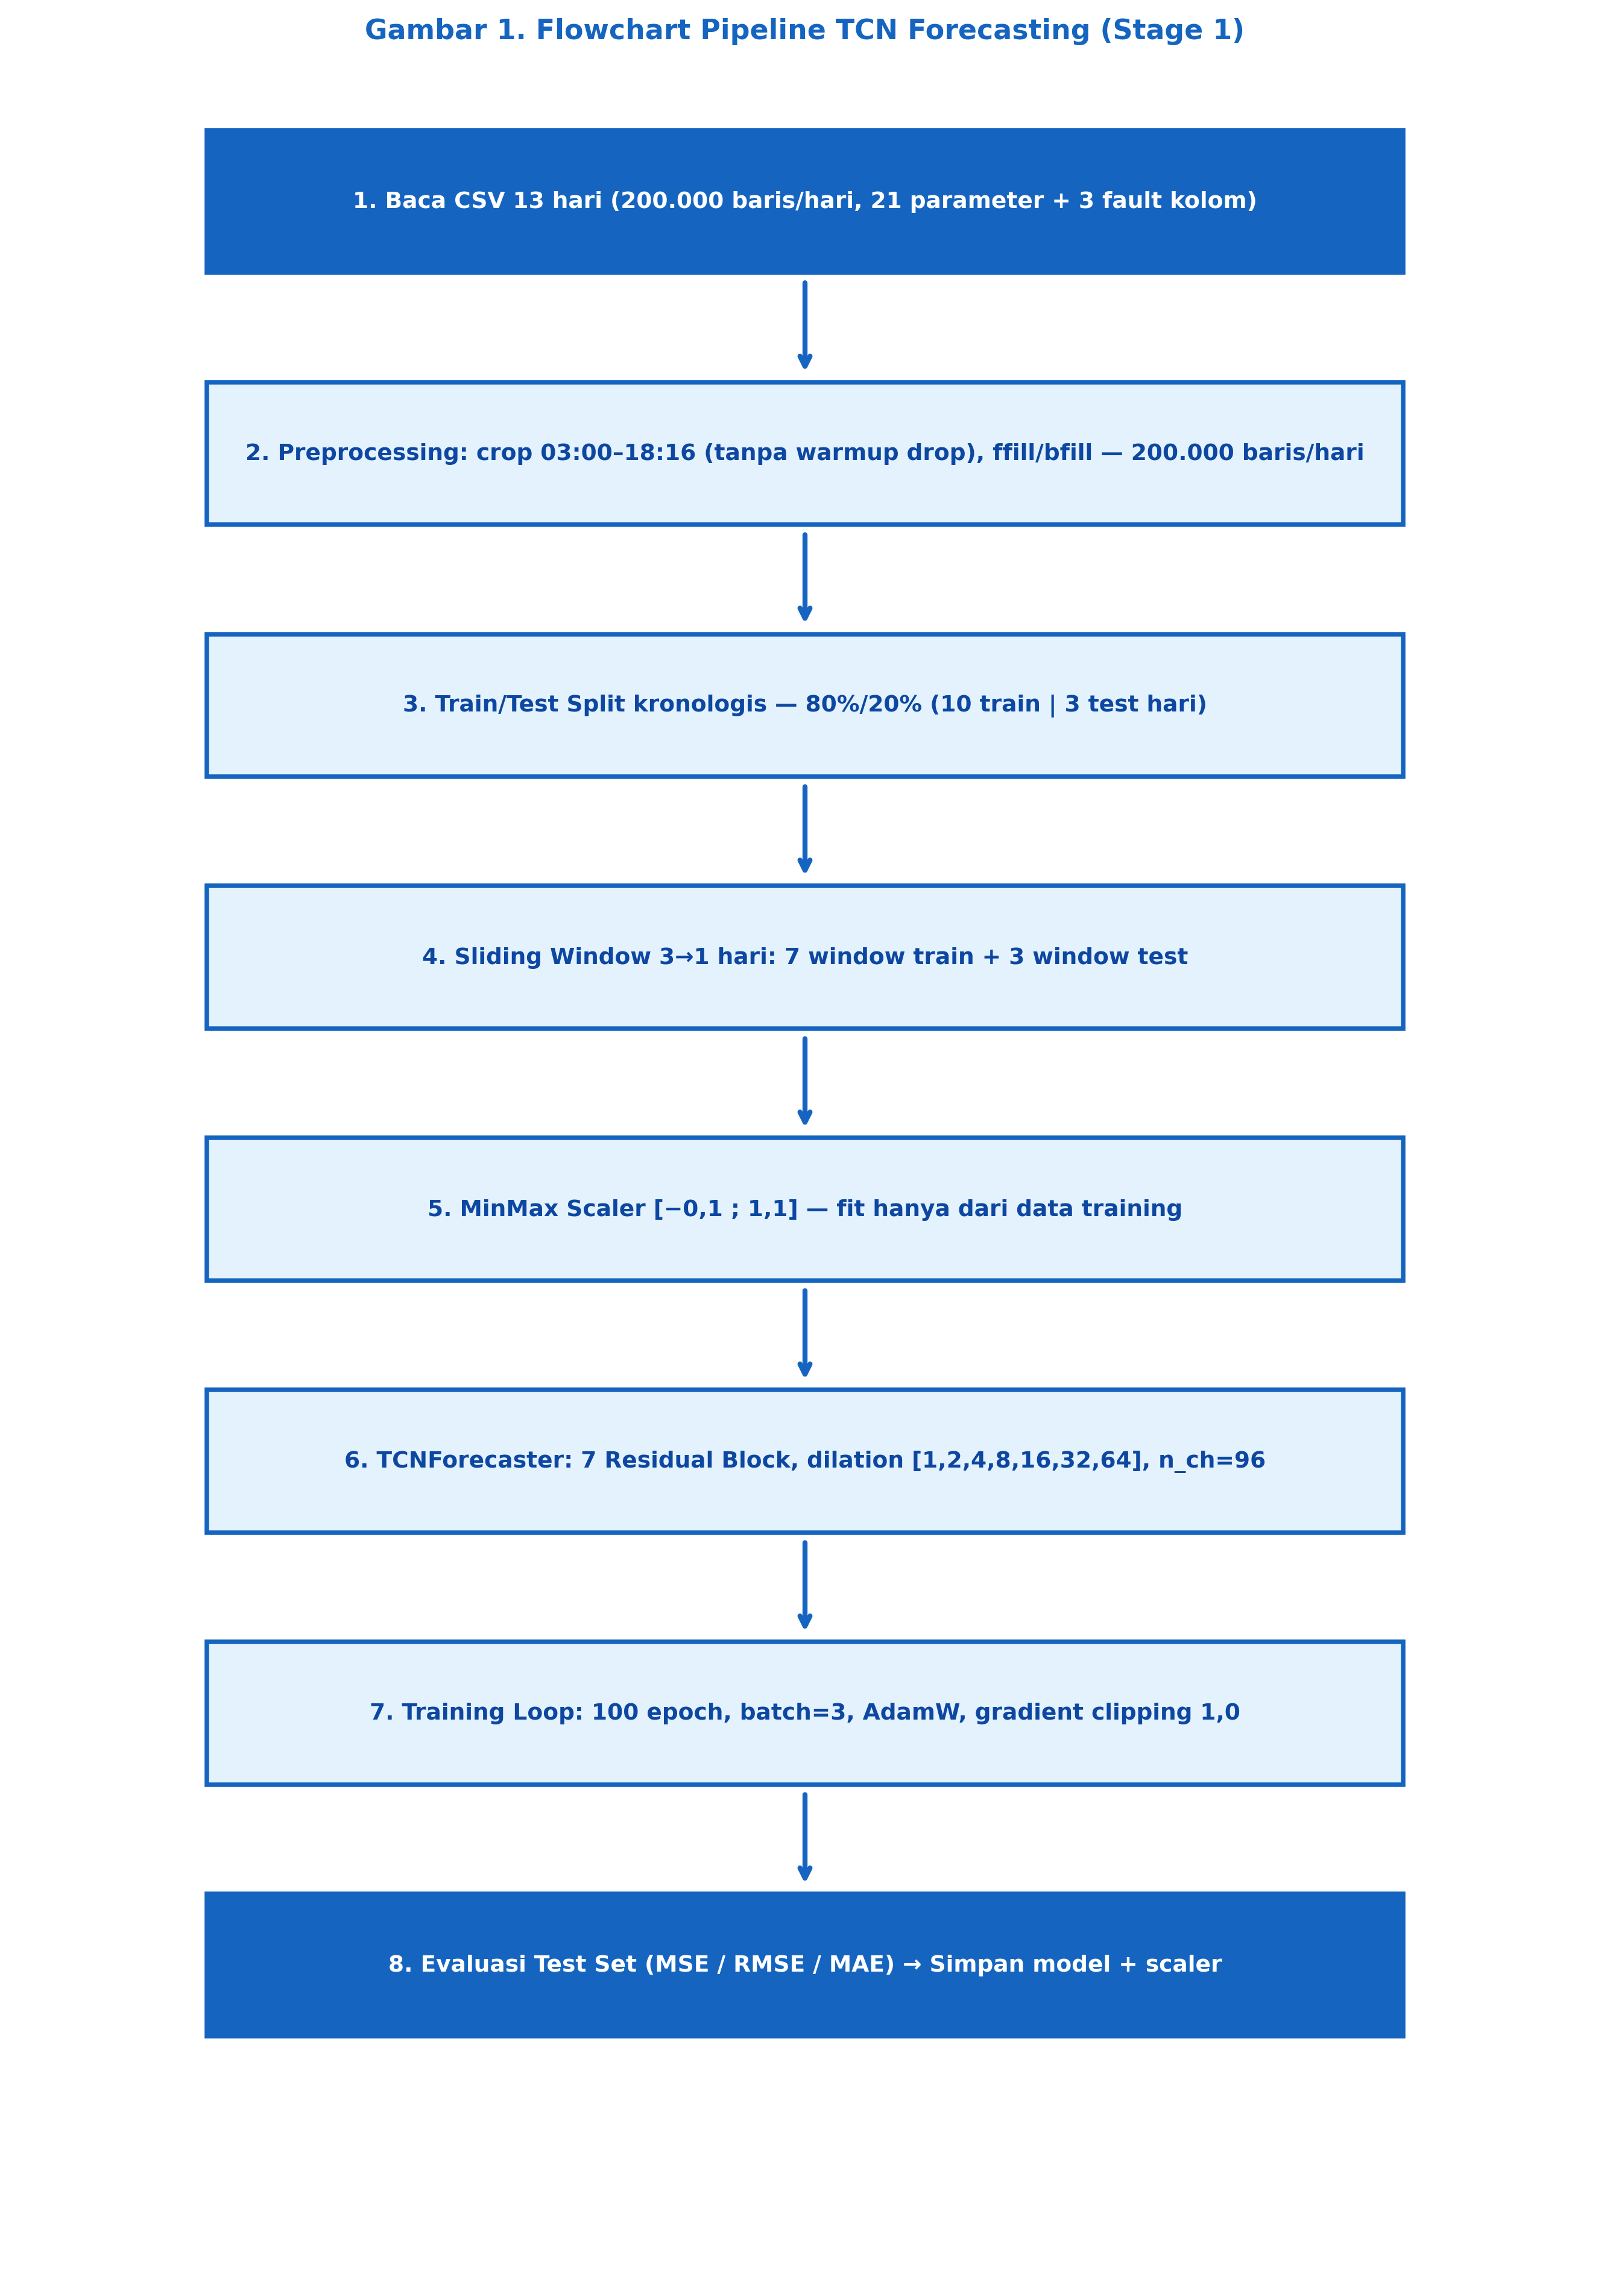
\includegraphics[width=0.95\linewidth]{jurnal_flowchart_stage1.png}
    \caption{Diagram alur (flowchart) pipeline Stage 1 — TCN Forecaster.}
    \label{fig:flow1}
\end{figure}

\begin{figure}[H]
    \centering
    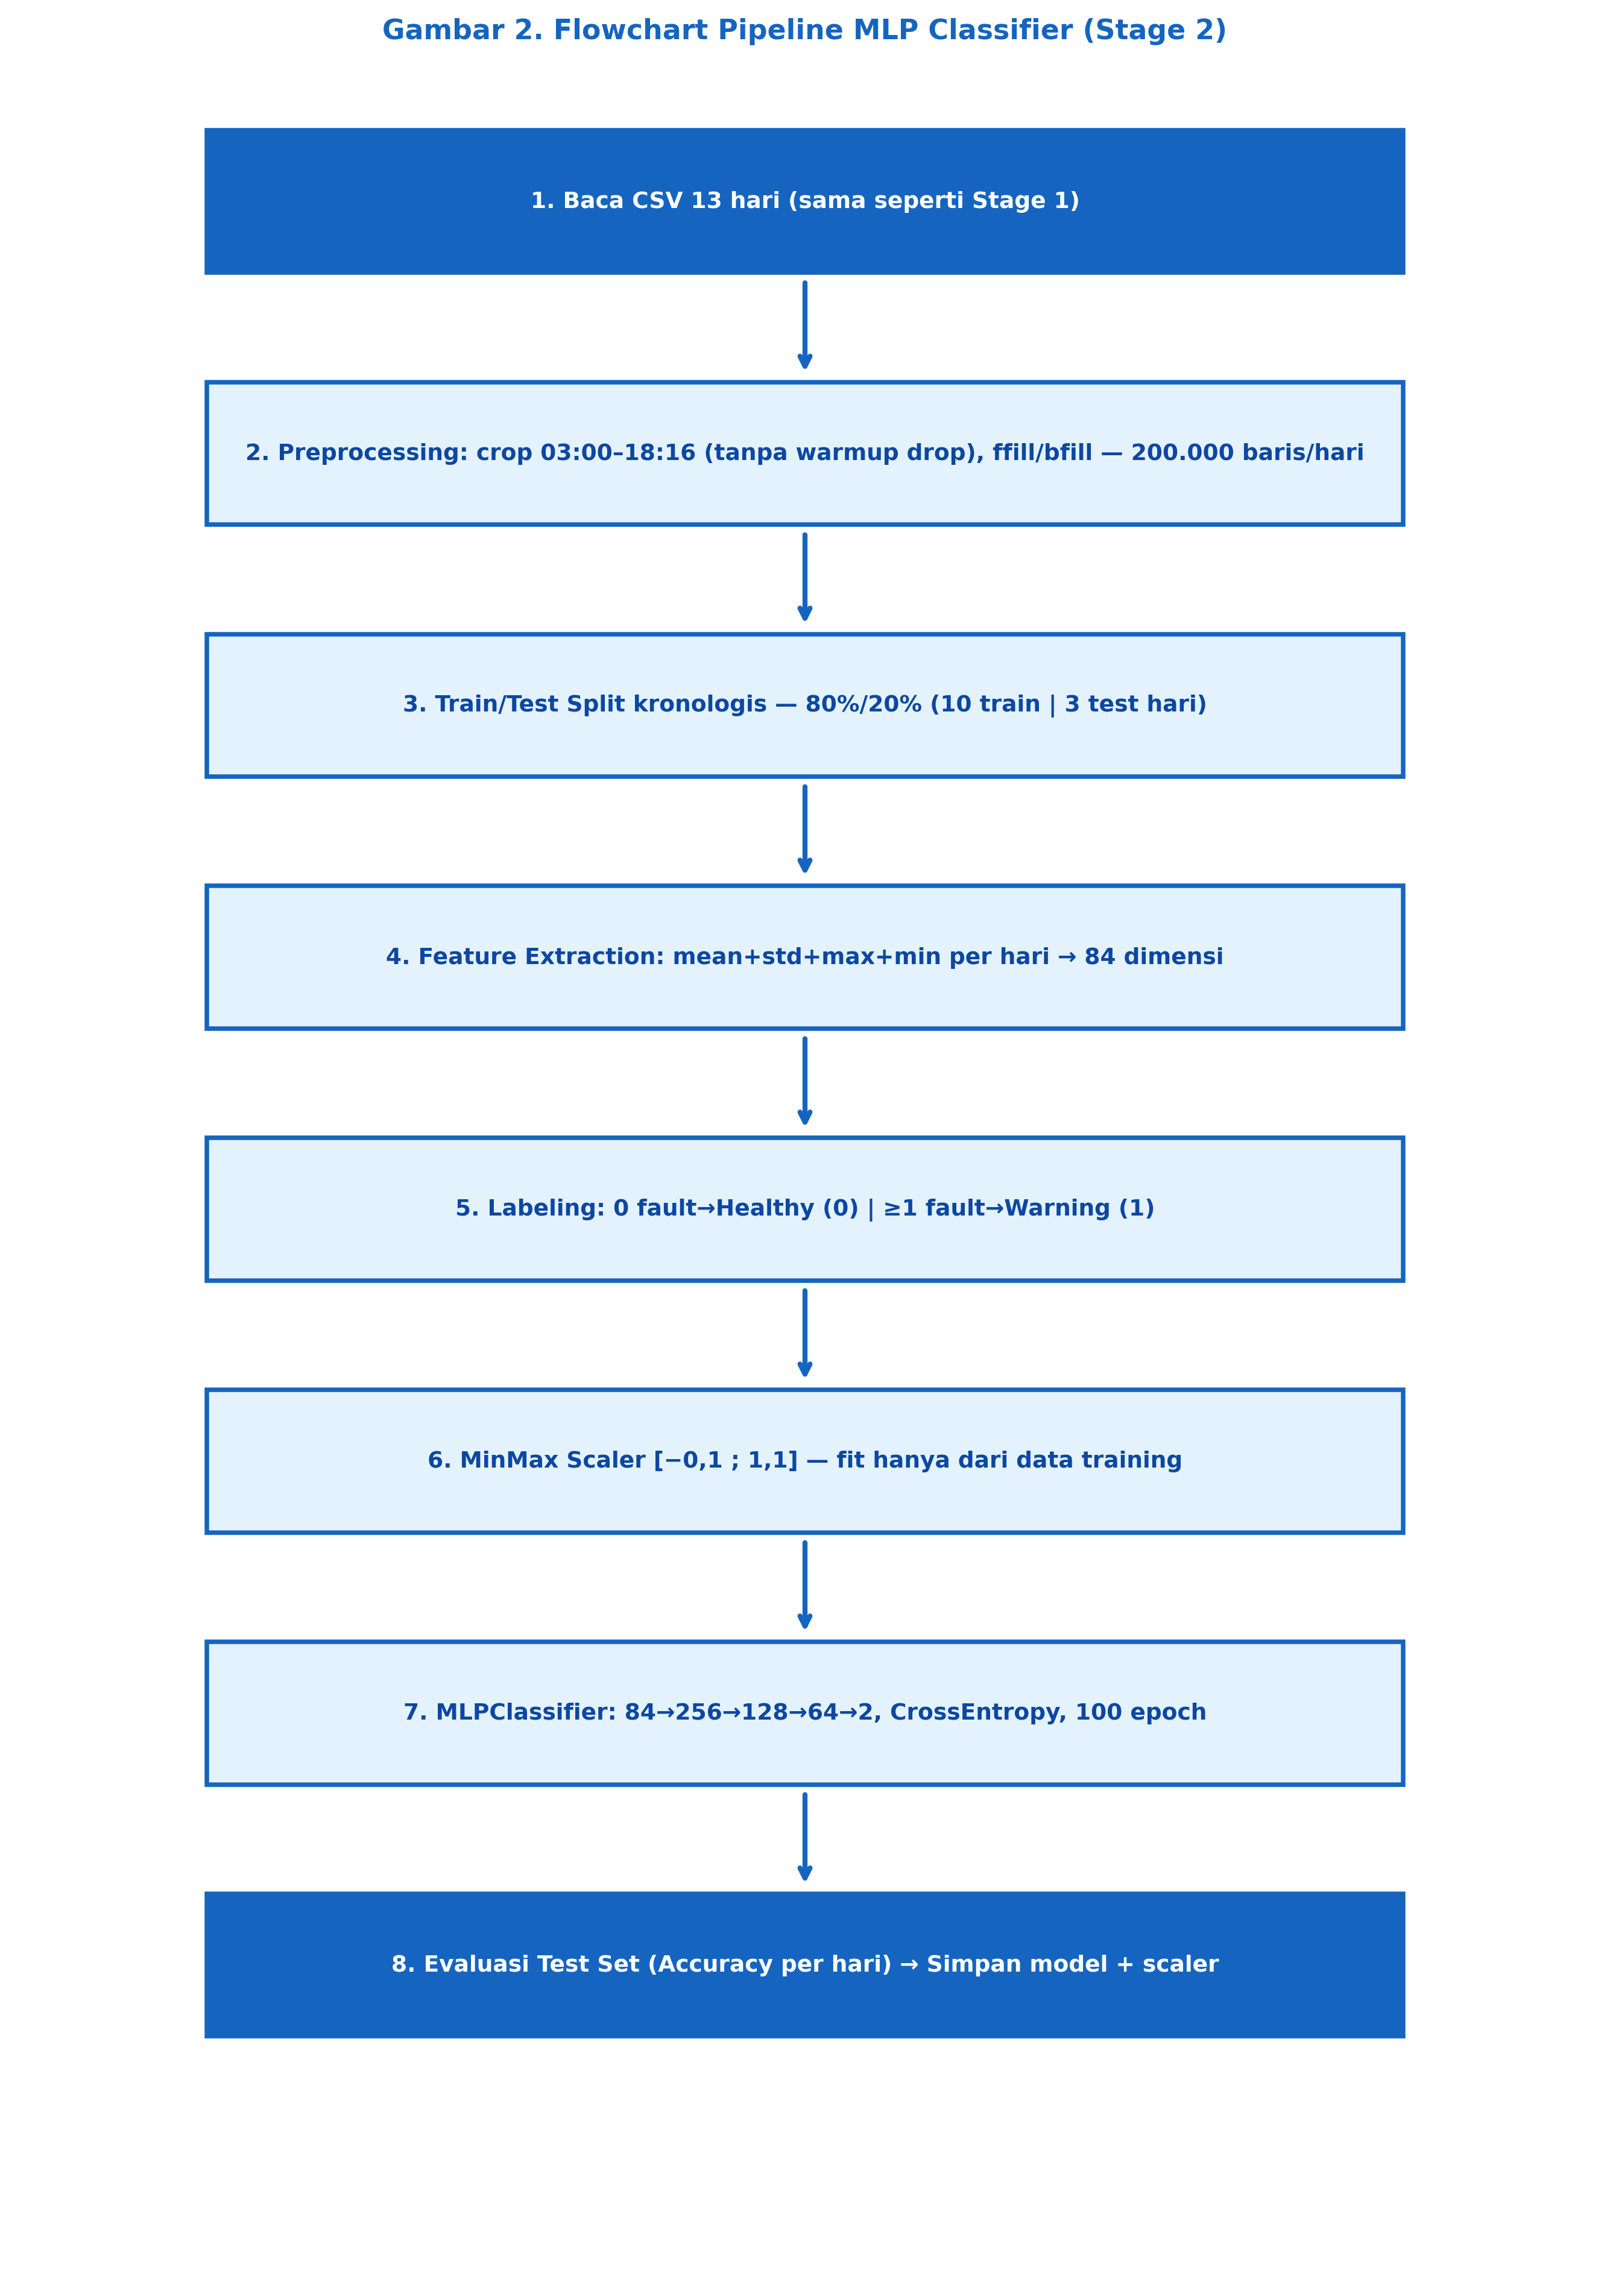
\includegraphics[width=0.95\linewidth]{jurnal_flowchart_stage2.png}
    \caption{Diagram alur (flowchart) pipeline Stage 2 — MLP Classifier.}
    \label{fig:flow2}
\end{figure}

\section{Dataset}
\subsection{Sumber dan Ringkasan Data}
\begin{table}[H]
    \centering
    \caption{Ringkasan dataset SIV TS27.}
    \begin{tabular}{ll}
        \toprule
        \textbf{Keterangan} & \textbf{Nilai} \\
        \midrule
        Total hari CSV valid & 37 hari \\
        Hari \textit{training} (80\%) & 29 hari \\
        Hari \textit{testing} (20\%) & 8 hari \\
        Baris per hari & 200.000 baris \\
        Total baris digunakan & 7.400.000 baris \\
        Jumlah parameter (fitur) & 21 parameter \\
        Window TCN (\textit{training}) & 26 window \\
        Window TCN (\textit{testing}) & 8 window \\
        Missing value handling & forward-fill (ffill) + backward-fill (bfill) \\
        \bottomrule
    \end{tabular}
\end{table}

Pembagian data mengikuti urutan waktu (\textit{chronological split}) untuk mencegah kebocoran data (\textit{data leakage}). Data \textit{training} mencakup Day 1--29 (02-01-2026 s/d 08-05-2026); data \textit{testing} mencakup Day 30--37 (09-05-2026 s/d 23-05-2026).

\subsection{Detail Pembagian Data}
\begin{longtable}{clcc}
    \toprule
    \textbf{Day} & \textbf{Tanggal} & \textbf{Set} & \textbf{Status Kesehatan} \\
    \midrule
    \endhead
    1  & 02012026 & Train & \warning \\
    2  & 10022026 & Train & \warning \\
    3  & 13022026 & Train & \healthy \\
    4  & 15022026 & Train & \healthy \\
    5  & 19022026 & Train & \healthy \\
    6  & 23022026 & Train & \healthy \\
    7  & 25022026 & Train & \healthy \\
    8  & 01032026 & Train & \warning \\
    9  & 07032026 & Train & \healthy \\
    10 & 22032026 & Train & \warning \\
    11 & 28032026 & Train & \healthy \\
    12 & 08042026 & Train & \healthy \\
    13 & 09042026 & Train & \healthy \\
    14 & 11042026 & Train & \healthy \\
    15 & 12042026 & Train & \healthy \\
    16 & 15042026 & Train & \healthy \\
    17 & 16042026 & Train & \healthy \\
    18 & 17042026 & Train & \healthy \\
    19 & 19042026 & Train & \healthy \\
    20 & 21042026 & Train & \warning \\
    21 & 22042026 & Train & \healthy \\
    22 & 23042026 & Train & \warning \\
    23 & 24042026 & Train & \healthy \\
    24 & 27042026 & Train & \warning \\
    25 & 04052026 & Train & \healthy \\
    26 & 05052026 & Train & \warning \\
    27 & 06052026 & Train & \warning \\
    28 & 07052026 & Train & \healthy \\
    29 & 08052026 & Train & \healthy \\
    30 & 09052026 & Test  & \healthy \\
    31 & 14052026 & Test  & \warning \\
    32 & 15052026 & Test  & \healthy \\
    33 & 16052026 & Test  & \healthy \\
    34 & 17052026 & Test  & \healthy \\
    35 & 20052026 & Test  & \warning \\
    36 & 22052026 & Test  & \warning \\
    37 & 23052026 & Test  & \healthy \\
    \bottomrule
    \caption{Detail 37 hari data beserta pembagian set dan status kesehatan aktual.}
    \label{tab:days}
\end{longtable}

\textbf{Distribusi label keseluruhan:} 25 hari \healthy\ (67,6\%), 12 hari \warning\ (32,4\%).

\begin{figure}[H]
    \centering
    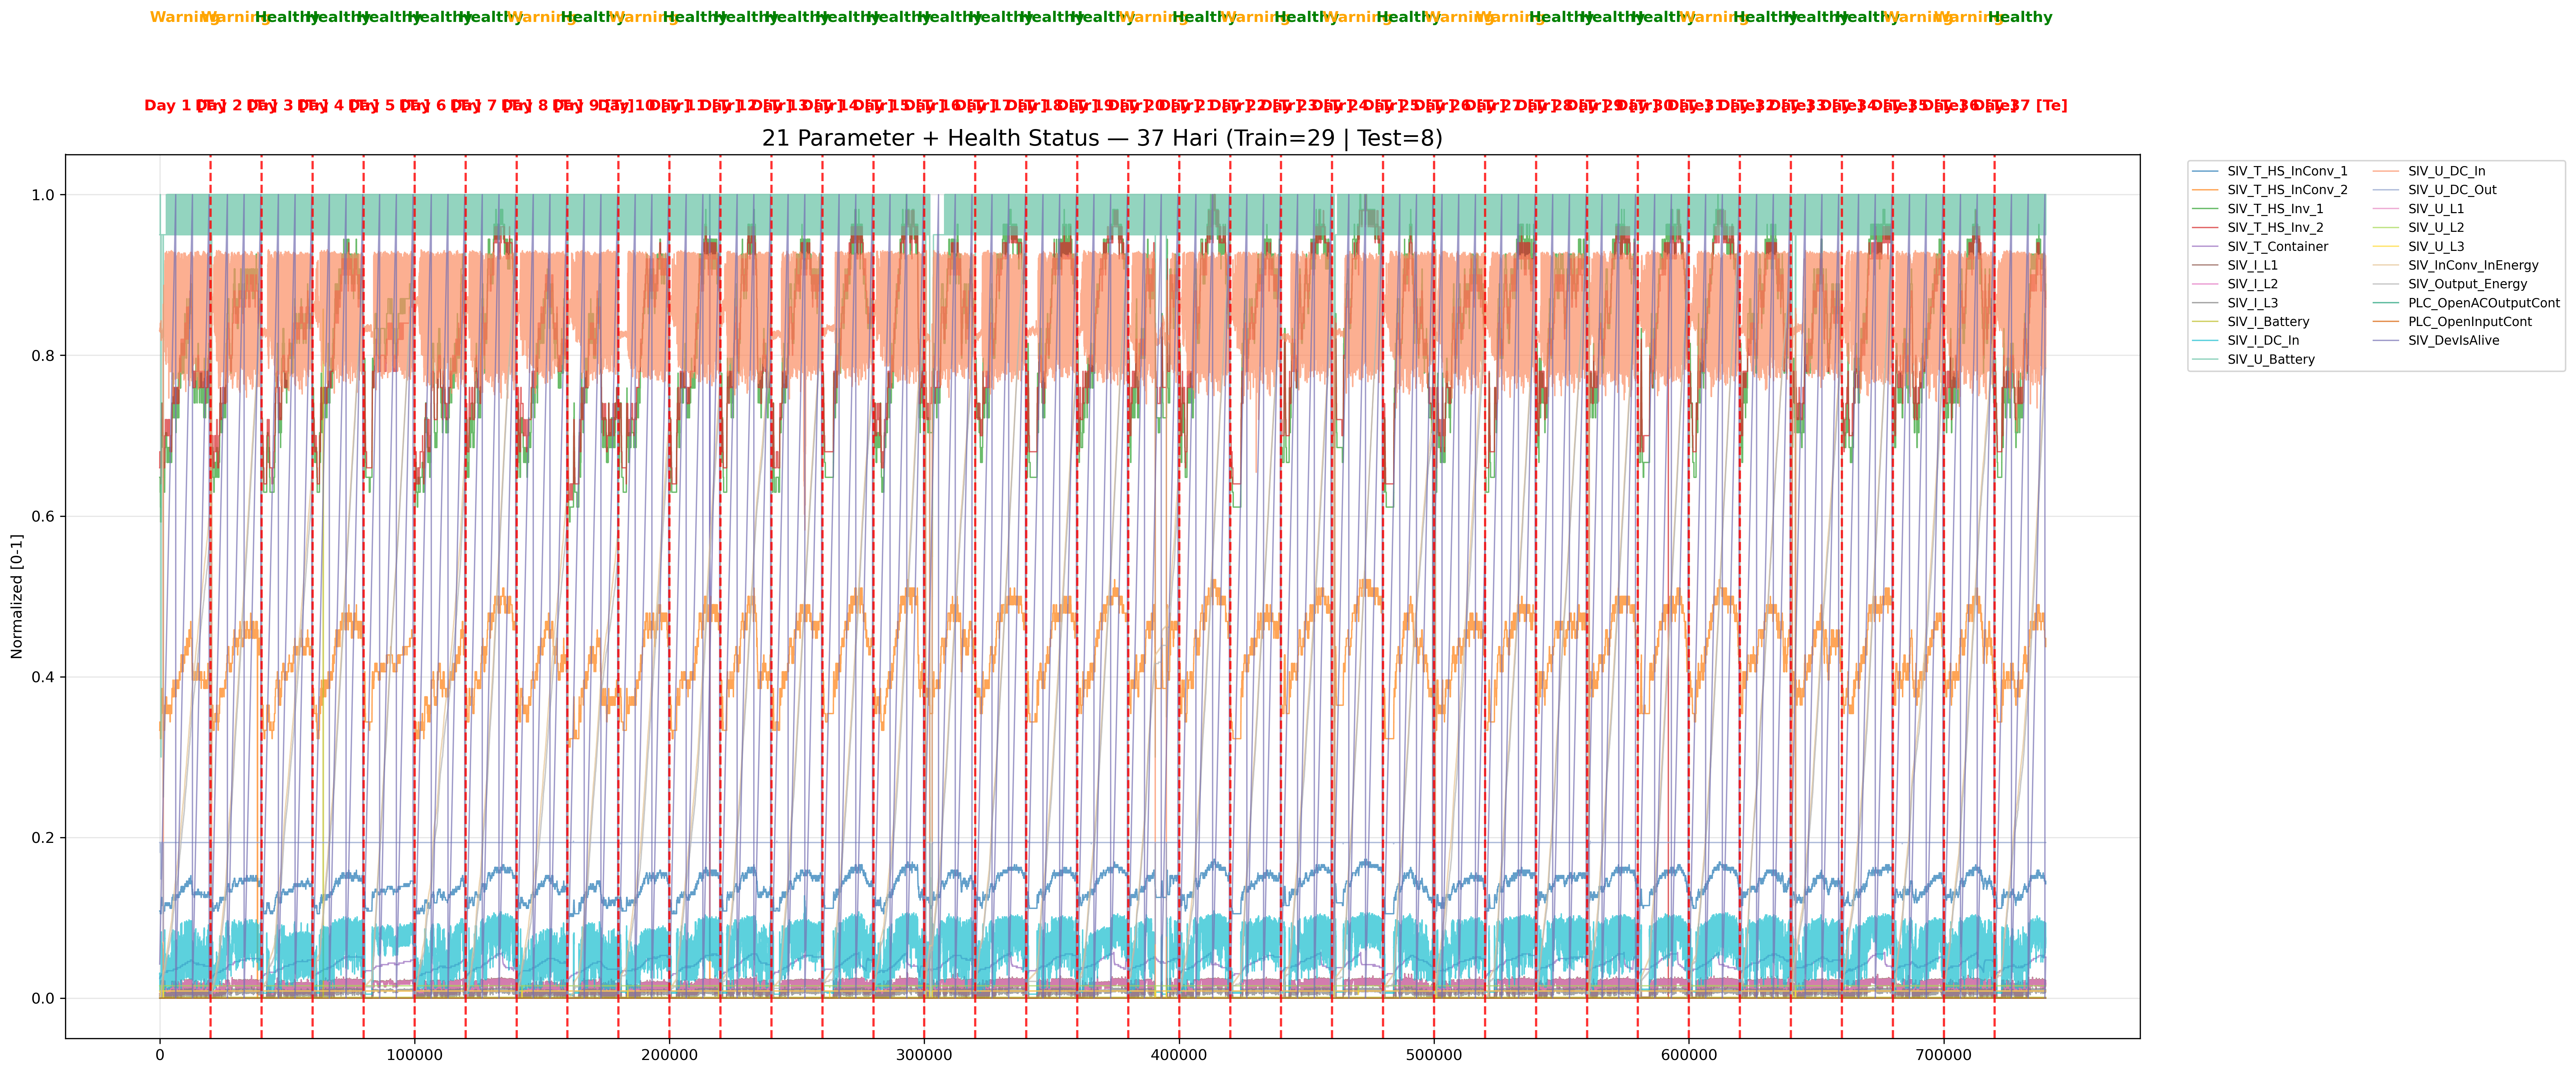
\includegraphics[width=\linewidth]{plot_all_parameters_TCN.png}
    \caption{Plot 21 parameter sensor untuk seluruh hari dataset.}
    \label{fig:allparam}
\end{figure}

\section{Preprocessing dan Normalisasi}
\subsection{Normalisasi Min-Max}
Seluruh 21 parameter dinormalisasi menggunakan \textbf{Min-Max Scaler} ke rentang $[-0,1;\ 1,1]$. Scaler di-\textit{fit} hanya pada 29 hari data \textit{training} untuk mencegah kebocoran data.

\begin{longtable}{lrr}
    \toprule
    \textbf{Parameter} & \textbf{Min Data} & \textbf{Max Data} \\
    \midrule
    \endhead
    SIV\_T\_HS\_InConv\_1   & 0,0000   & 295,0000 \\
    SIV\_T\_HS\_InConv\_2   & 0,0000   & 96,0000 \\
    SIV\_T\_HS\_Inv\_1      & 31,0000  & 54,0000 \\
    SIV\_T\_HS\_Inv\_2      & 31,0000  & 50,0000 \\
    SIV\_T\_Container       & 30,0000  & 557,0000 \\
    SIV\_I\_L1              & 0,0000   & 4144,0000 \\
    SIV\_I\_L2              & 0,0000   & 126,0000 \\
    SIV\_I\_L3              & 0,0000   & 8198,0000 \\
    SIV\_I\_Battery         & -33,0000 & 24800,0000 \\
    SIV\_I\_DC\_In          & 0,0000   & 544,0000 \\
    SIV\_U\_Battery         & 94,0000  & 114,0000 \\
    SIV\_U\_DC\_In          & 0,0000   & 936,0000 \\
    SIV\_U\_DC\_Out         & 3,0000   & 127,0000 \\
    SIV\_U\_L1              & 0,0000   & 24768,0000 \\
    SIV\_U\_L2              & 0,0000   & 14272,0000 \\
    SIV\_U\_L3              & 0,0000   & 24603,0000 \\
    SIV\_InConv\_InEnergy   & 0,0000   & 644,0000 \\
    SIV\_Output\_Energy     & 0,0000   & 574,0000 \\
    PLC\_OpenACOutputCont   & 0,0000   & 0,0000 \\
    PLC\_OpenInputCont      & 0,0000   & 0,0000 \\
    SIV\_DevIsAlive         & 0,0000   & 65535,0000 \\
    \bottomrule
    \caption{Rentang nilai (min--max) 21 parameter dari scaler training.}
    \label{tab:minmax}
\end{longtable}

\begin{figure}[H]
    \centering
    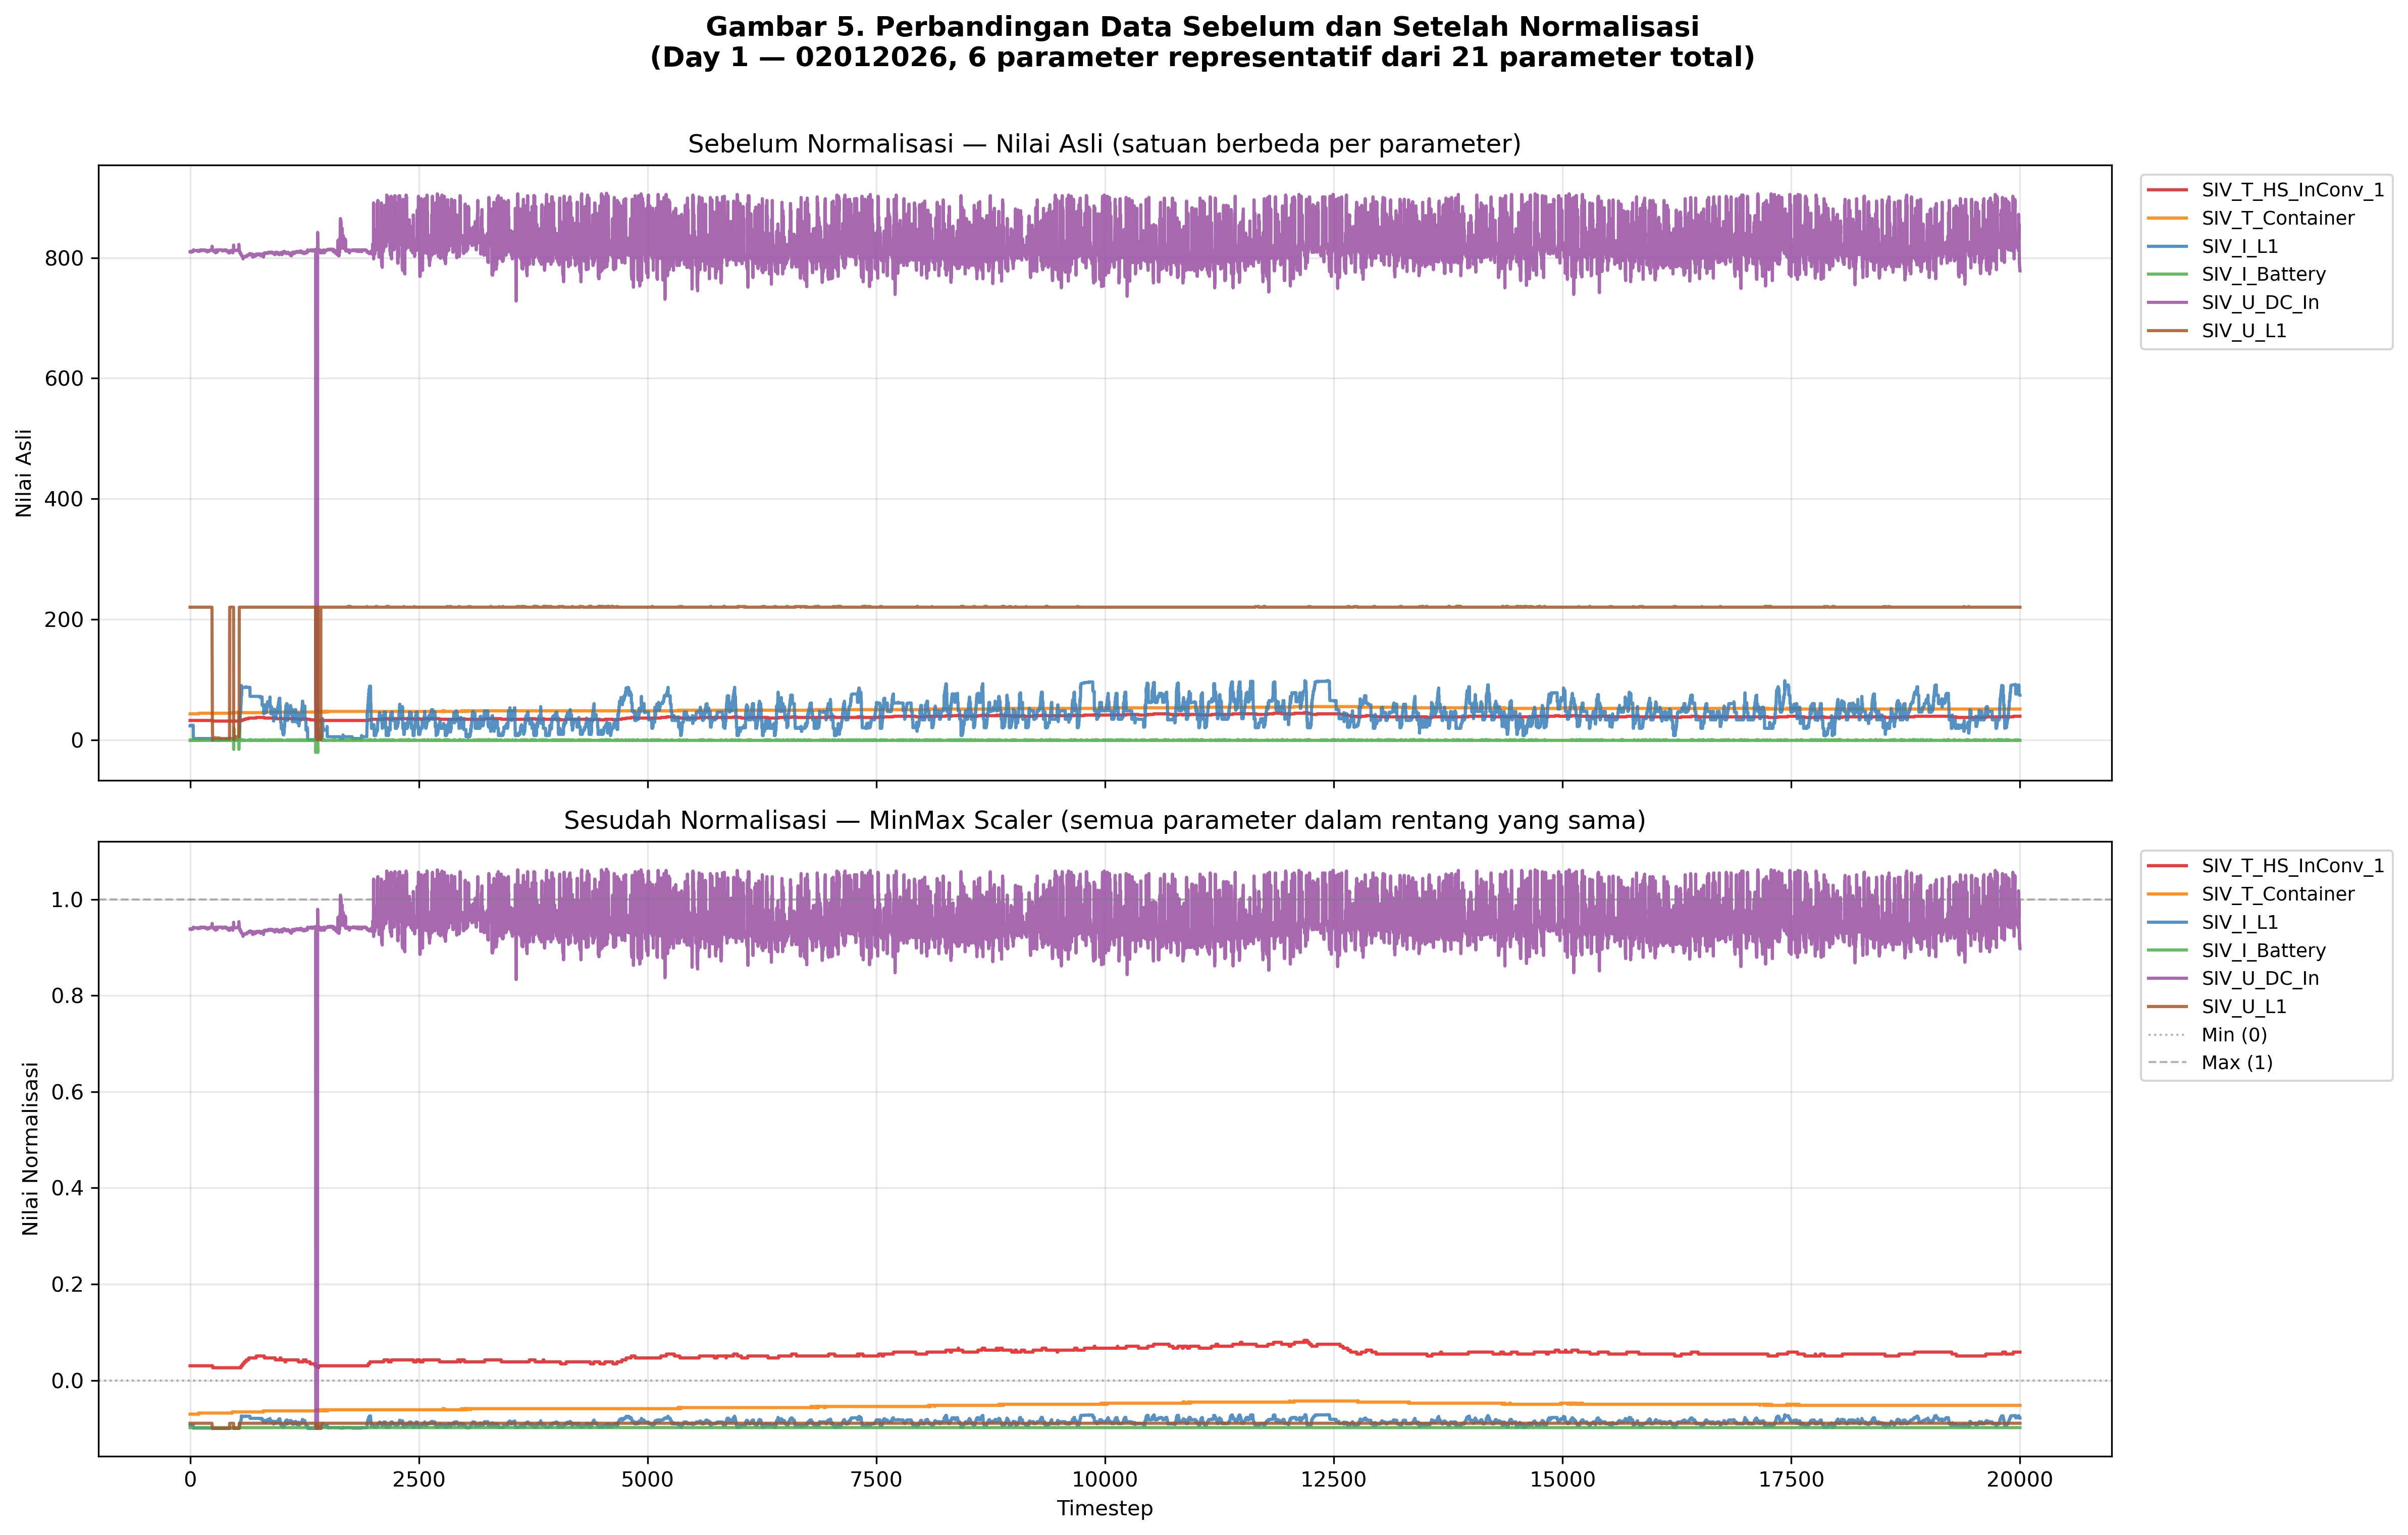
\includegraphics[width=0.9\linewidth]{jurnal_normalisasi_comparison.png}
    \caption{Perbandingan data sebelum vs sesudah normalisasi Min-Max.}
    \label{fig:norm}
\end{figure}

\subsection{Skema Sliding Window}
Sequence input-output dibentuk menggunakan skema \textit{sliding window} 3 hari input $\rightarrow$ 1 hari target (H+1), digeser satu hari setiap langkah.

\begin{figure}[H]
    \centering
    \includegraphics[width=0.8\linewidth]{jurnal_sliding_window.png}
    \caption{Skema sliding window: 3 hari input memprediksi 1 hari target berikutnya.}
    \label{fig:slidewin}
\end{figure}

\section{Arsitektur Model}
\subsection{Stage 1 — TCN Forecaster}
\begin{table}[H]
    \centering
    \caption{Arsitektur TCN (Temporal Convolutional Network).}
    \begin{tabular}{ll}
        \toprule
        \textbf{Komponen} & \textbf{Spesifikasi} \\
        \midrule
        Jumlah Residual Block & 7 \\
        Dilation Factors & [1, 2, 4, 8, 16, 32, 64] \\
        Hidden Channel ($n_{ch}$) & 96 \\
        Kernel Size & 3 \\
        Input Window & 3 hari = 600.000 timestep \\
        Output Horizon & H+1 = 200.000 timestep (1 hari) \\
        Input Shape & (batch, 600000, 21) \\
        Output Shape & (batch, 200000, 21) \\
        \bottomrule
    \end{tabular}
\end{table}

\begin{table}[H]
    \centering
    \caption{Hyperparameter training Stage 1 (TCN Forecaster).}
    \begin{tabular}{ll}
        \toprule
        \textbf{Hyperparameter} & \textbf{Nilai} \\
        \midrule
        Optimizer & AdamW \\
        Learning Rate & 0,001 \\
        Batch Size & 3 \\
        Epoch & 100 \\
        Loss Function & Mean Squared Error (MSE) \\
        Gradient Clipping & 1,0 \\
        Dropout & 0,3 \\
        Weight Decay & 1e-5 \\
        Scheduler & ReduceLROnPlateau (factor=0,5, patience=30) \\
        \bottomrule
    \end{tabular}
\end{table}

\subsection{Stage 2 — MLP Classifier}
Hasil \textit{forecast} Stage 1 diringkas menjadi \textbf{84 fitur statistik} (\textit{mean}, \textit{std}, \textit{min}, \textit{max} $\times$ 21 parameter) sebagai input MLP Classifier.

\begin{table}[H]
    \centering
    \caption{Arsitektur MLP Classifier.}
    \begin{tabular}{ll}
        \toprule
        \textbf{Layer} & \textbf{Spesifikasi} \\
        \midrule
        Input Layer   & 84 neuron \\
        Hidden Layer 1 & 256 neuron + LayerNorm + ReLU + Dropout \\
        Hidden Layer 2 & 128 neuron + LayerNorm + ReLU + Dropout \\
        Hidden Layer 3 & 64 neuron + LayerNorm + ReLU + Dropout \\
        Output Layer  & 2 neuron (Softmax) — Healthy / Warning \\
        \bottomrule
    \end{tabular}
\end{table}

\begin{table}[H]
    \centering
    \caption{Hyperparameter training Stage 2 (MLP Classifier).}
    \begin{tabular}{ll}
        \toprule
        \textbf{Hyperparameter} & \textbf{Nilai} \\
        \midrule
        Optimizer & AdamW \\
        Learning Rate & 0,001 \\
        Batch Size & 3 \\
        Epoch & 100 \\
        Loss Function & Cross-Entropy Loss \\
        Class Weight & Healthy = 0,5, Warning = 2,5 \\
        Dropout & 0,3 \\
        Weight Decay & 1e-5 \\
        Scheduler & ReduceLROnPlateau (factor=0,5, patience=30) \\
        \bottomrule
    \end{tabular}
\end{table}

\section{Prosedur Eksperimen}
\begin{enumerate}
    \item Pengumpulan data mentah 37 hari (masing-masing 200.000 baris, 21 parameter).
    \item \textit{Preprocessing}: penanganan \textit{missing value} (ffill + bfill).
    \item \textit{Split} data \textit{training}/\textit{testing} secara kronologis (29/8 hari).
    \item Normalisasi Min-Max (\textit{fit} pada data \textit{training}).
    \item Pembentukan \textit{sliding window} (3 hari input $\to$ 1 hari target).
    \item Training Stage 1 (TCN Forecaster) selama 100 epoch.
    \item Ekstraksi 84 fitur statistik dari hasil \textit{forecast} Stage 1.
    \item Training Stage 2 (MLP Classifier) selama 100 epoch.
    \item Evaluasi kedua model pada data \textit{training} dan \textit{testing}.
    \item Inference akhir (training inference dan testing/future inference).
\end{enumerate}

\newpage
% ============================================================
\chapter{HASIL DAN PEMBAHASAN}
% ============================================================

\section{Hasil Training Stage 1 — TCN Forecaster}
Loss (MSE) menurun dari \textbf{0,3568467} (35,68\%) pada epoch 1 menjadi \textbf{0,0120068} (1,20\%) pada epoch 100, atau penurunan total sebesar \textbf{96,6\%}.

\begin{figure}[H]
    \centering
    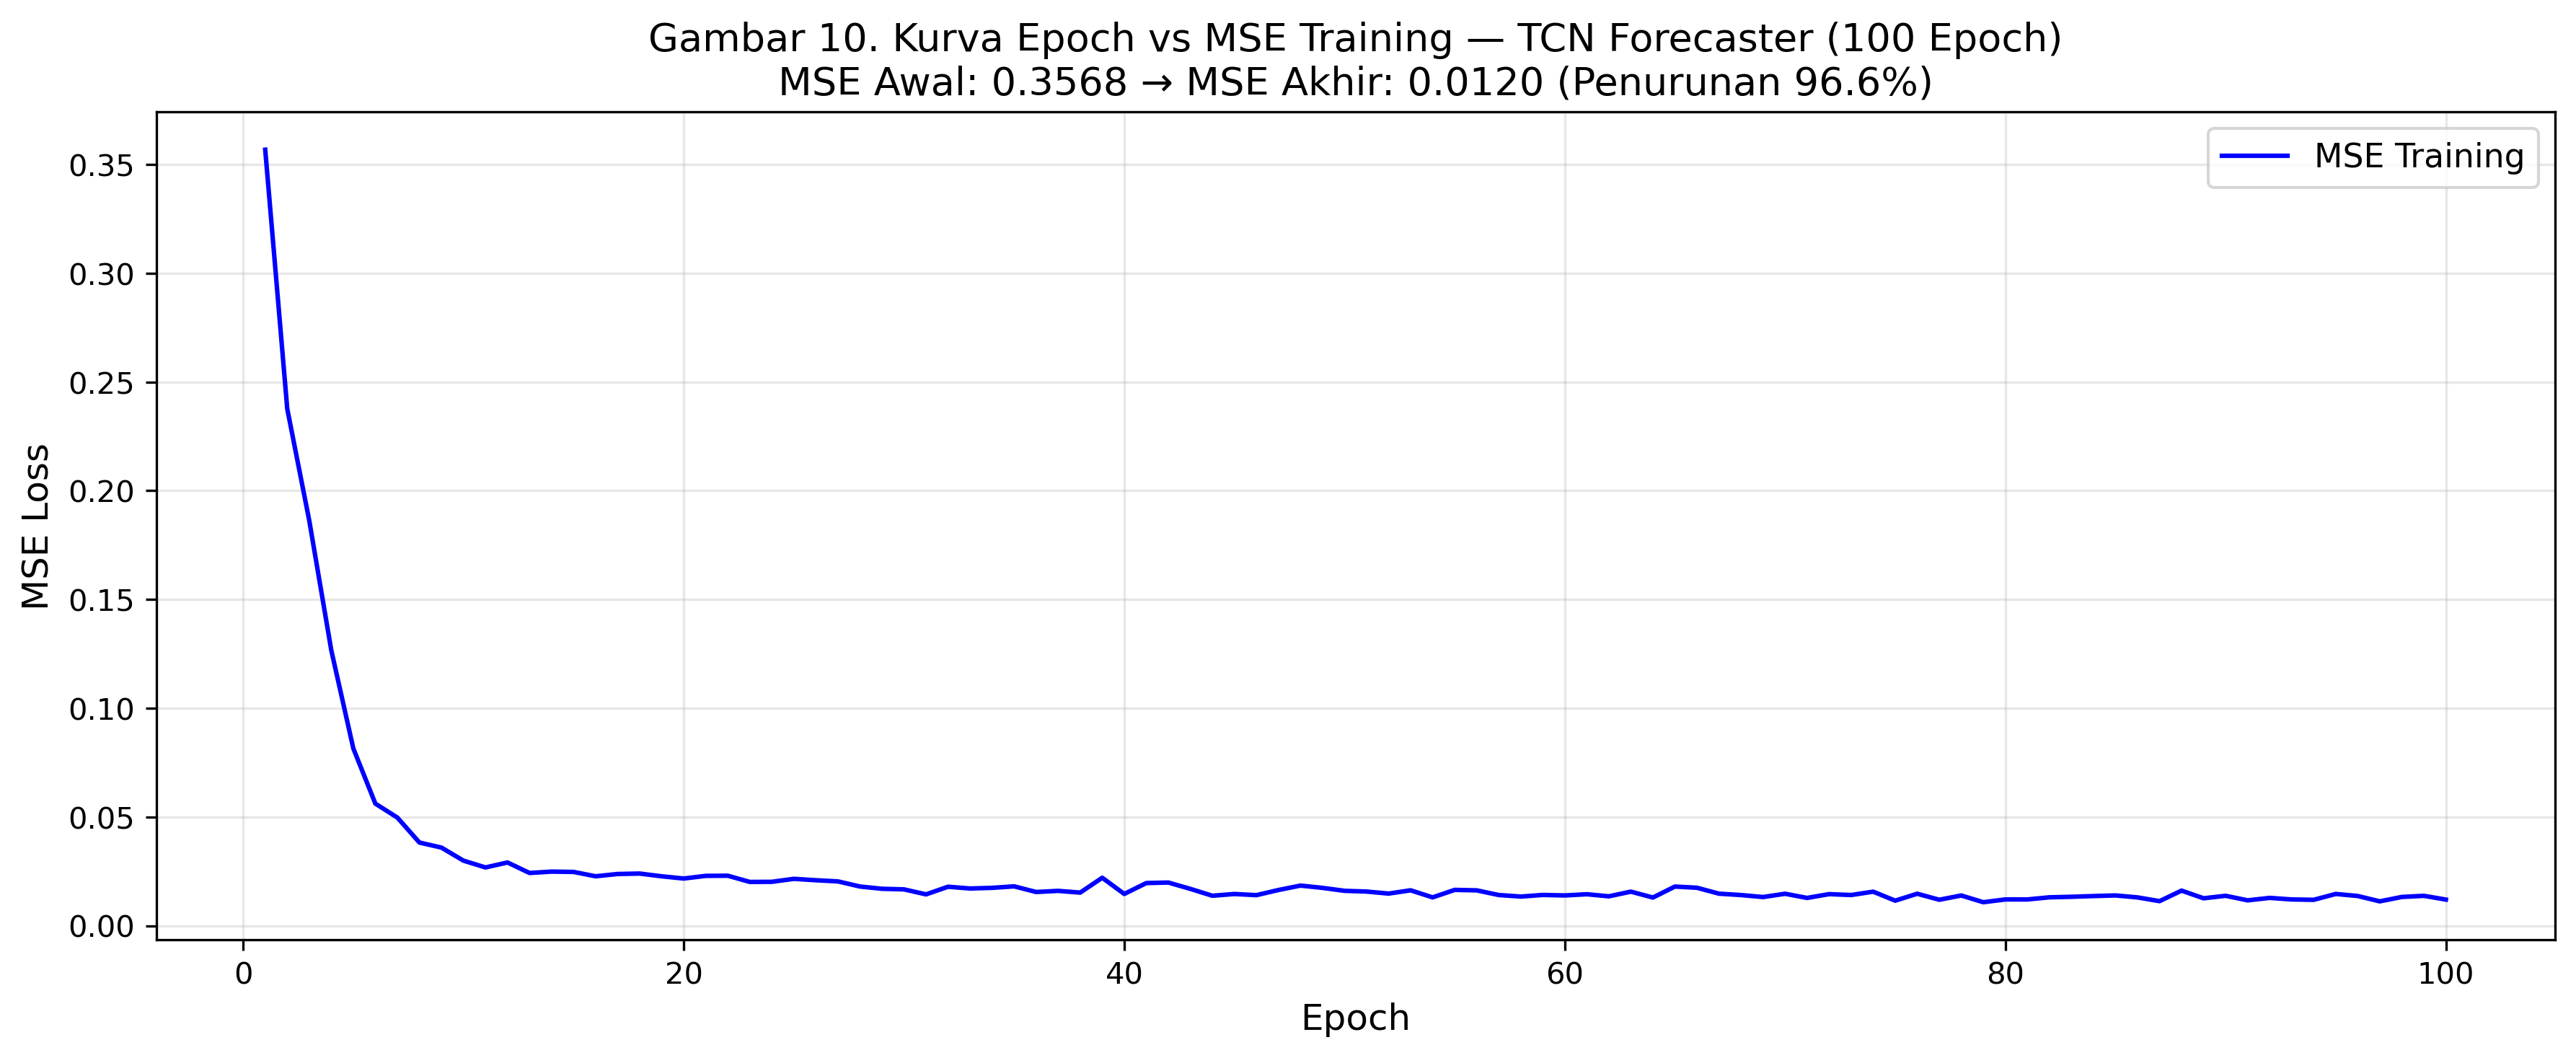
\includegraphics[width=0.8\linewidth]{jurnal_kurva_loss_stage1.png}
    \caption{Kurva Epoch vs MSE selama training Stage 1 (TCN Forecaster).}
    \label{fig:loss1}
\end{figure}

\begin{table}[H]
    \centering
    \caption{Metrik evaluasi Stage 1 pada skala ternormalisasi $[-0,1;\ 1,1]$.}
    \begin{tabular}{lrr}
        \toprule
        \textbf{Metrik} & \textbf{Training Set (26 window)} & \textbf{Test Set (8 window)} \\
        \midrule
        MSE  & 0,008066 & 0,007446 \\
        RMSE & 0,089810 & 0,086292 \\
        MAE  & 0,046303 & 0,043340 \\
        MAPE & 44,83\%  & 42,43\% \\
        \bottomrule
    \end{tabular}
\end{table}

\noindent Selisih MSE train--test sangat kecil (0,00456), mengindikasikan model TCN \textbf{tidak mengalami overfitting} dan mampu generalisasi dengan baik terhadap data yang belum pernah dilihat.

\section{Hasil Training Stage 2 — MLP Classifier}
CE Loss menurun dari \textbf{1,005112} (epoch 1) menjadi \textbf{0,068207} (epoch 100) — penurunan \textbf{93,2\%}. Akurasi \textit{training} meningkat dari 66,67\% menjadi 96,30\%, bahkan mencapai 100\% pada banyak epoch di paruh kedua training.

\begin{figure}[H]
    \centering
    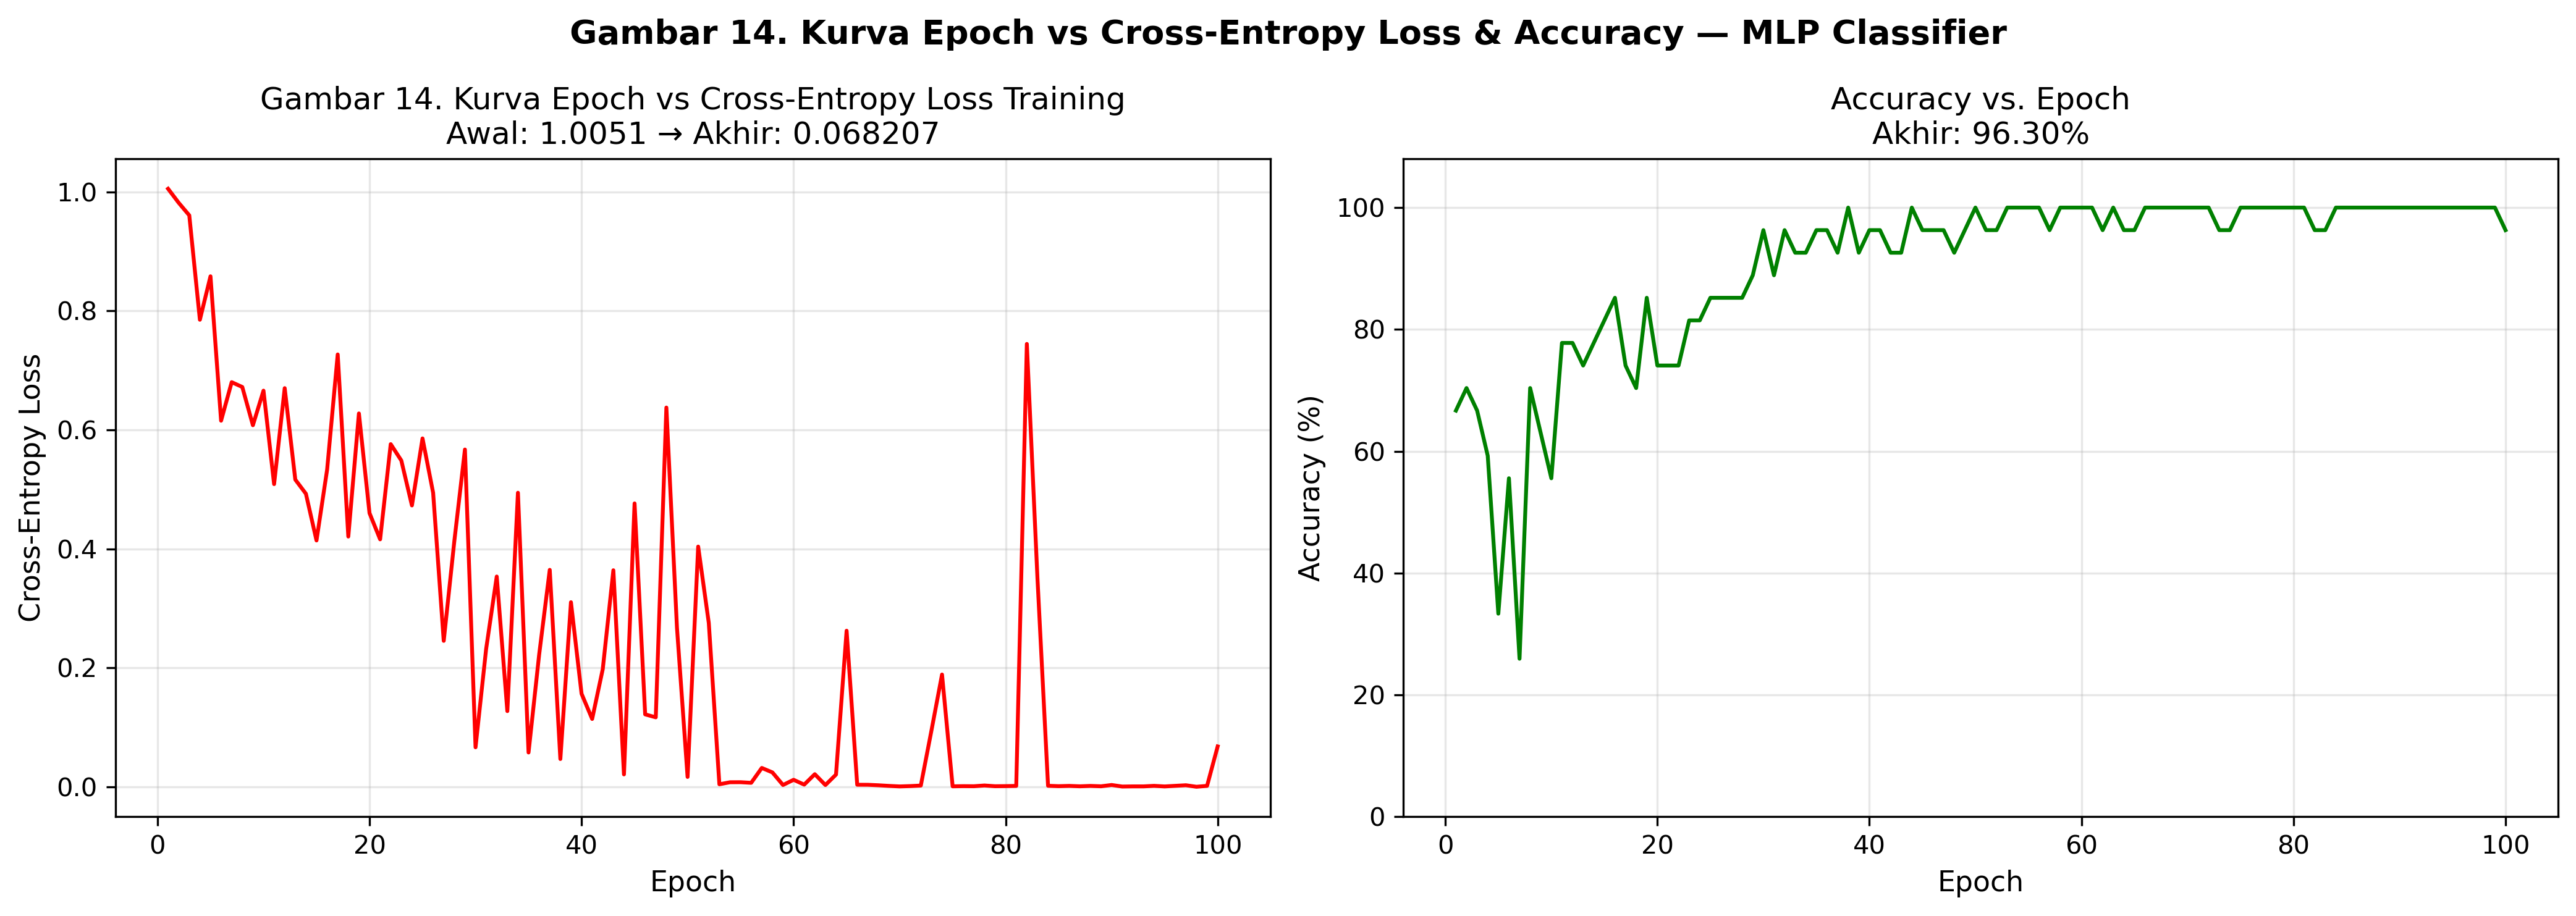
\includegraphics[width=0.8\linewidth]{jurnal_kurva_loss_acc_stage2.png}
    \caption{Kurva CE Loss dan Accuracy selama training Stage 2 (MLP Classifier).}
    \label{fig:loss2}
\end{figure}

\begin{table}[H]
    \centering
    \caption{Metrik evaluasi Stage 2 — Training Set (29 hari) vs Test Set (8 hari).}
    \begin{tabular}{lrr}
        \toprule
        \textbf{Metrik} & \textbf{Training} & \textbf{Testing} \\
        \midrule
        CE Loss   & 0,000223 & 5,903700 \\
        Accuracy  & 100,00\% & 62,50\% \\
        Precision & 100,00\% & 39,06\% \\
        Recall    & 100,00\% & 62,50\% \\
        F1-Score  & 100,00\% & 48,08\% \\
        \bottomrule
    \end{tabular}
\end{table}

\begin{figure}[H]
    \centering
    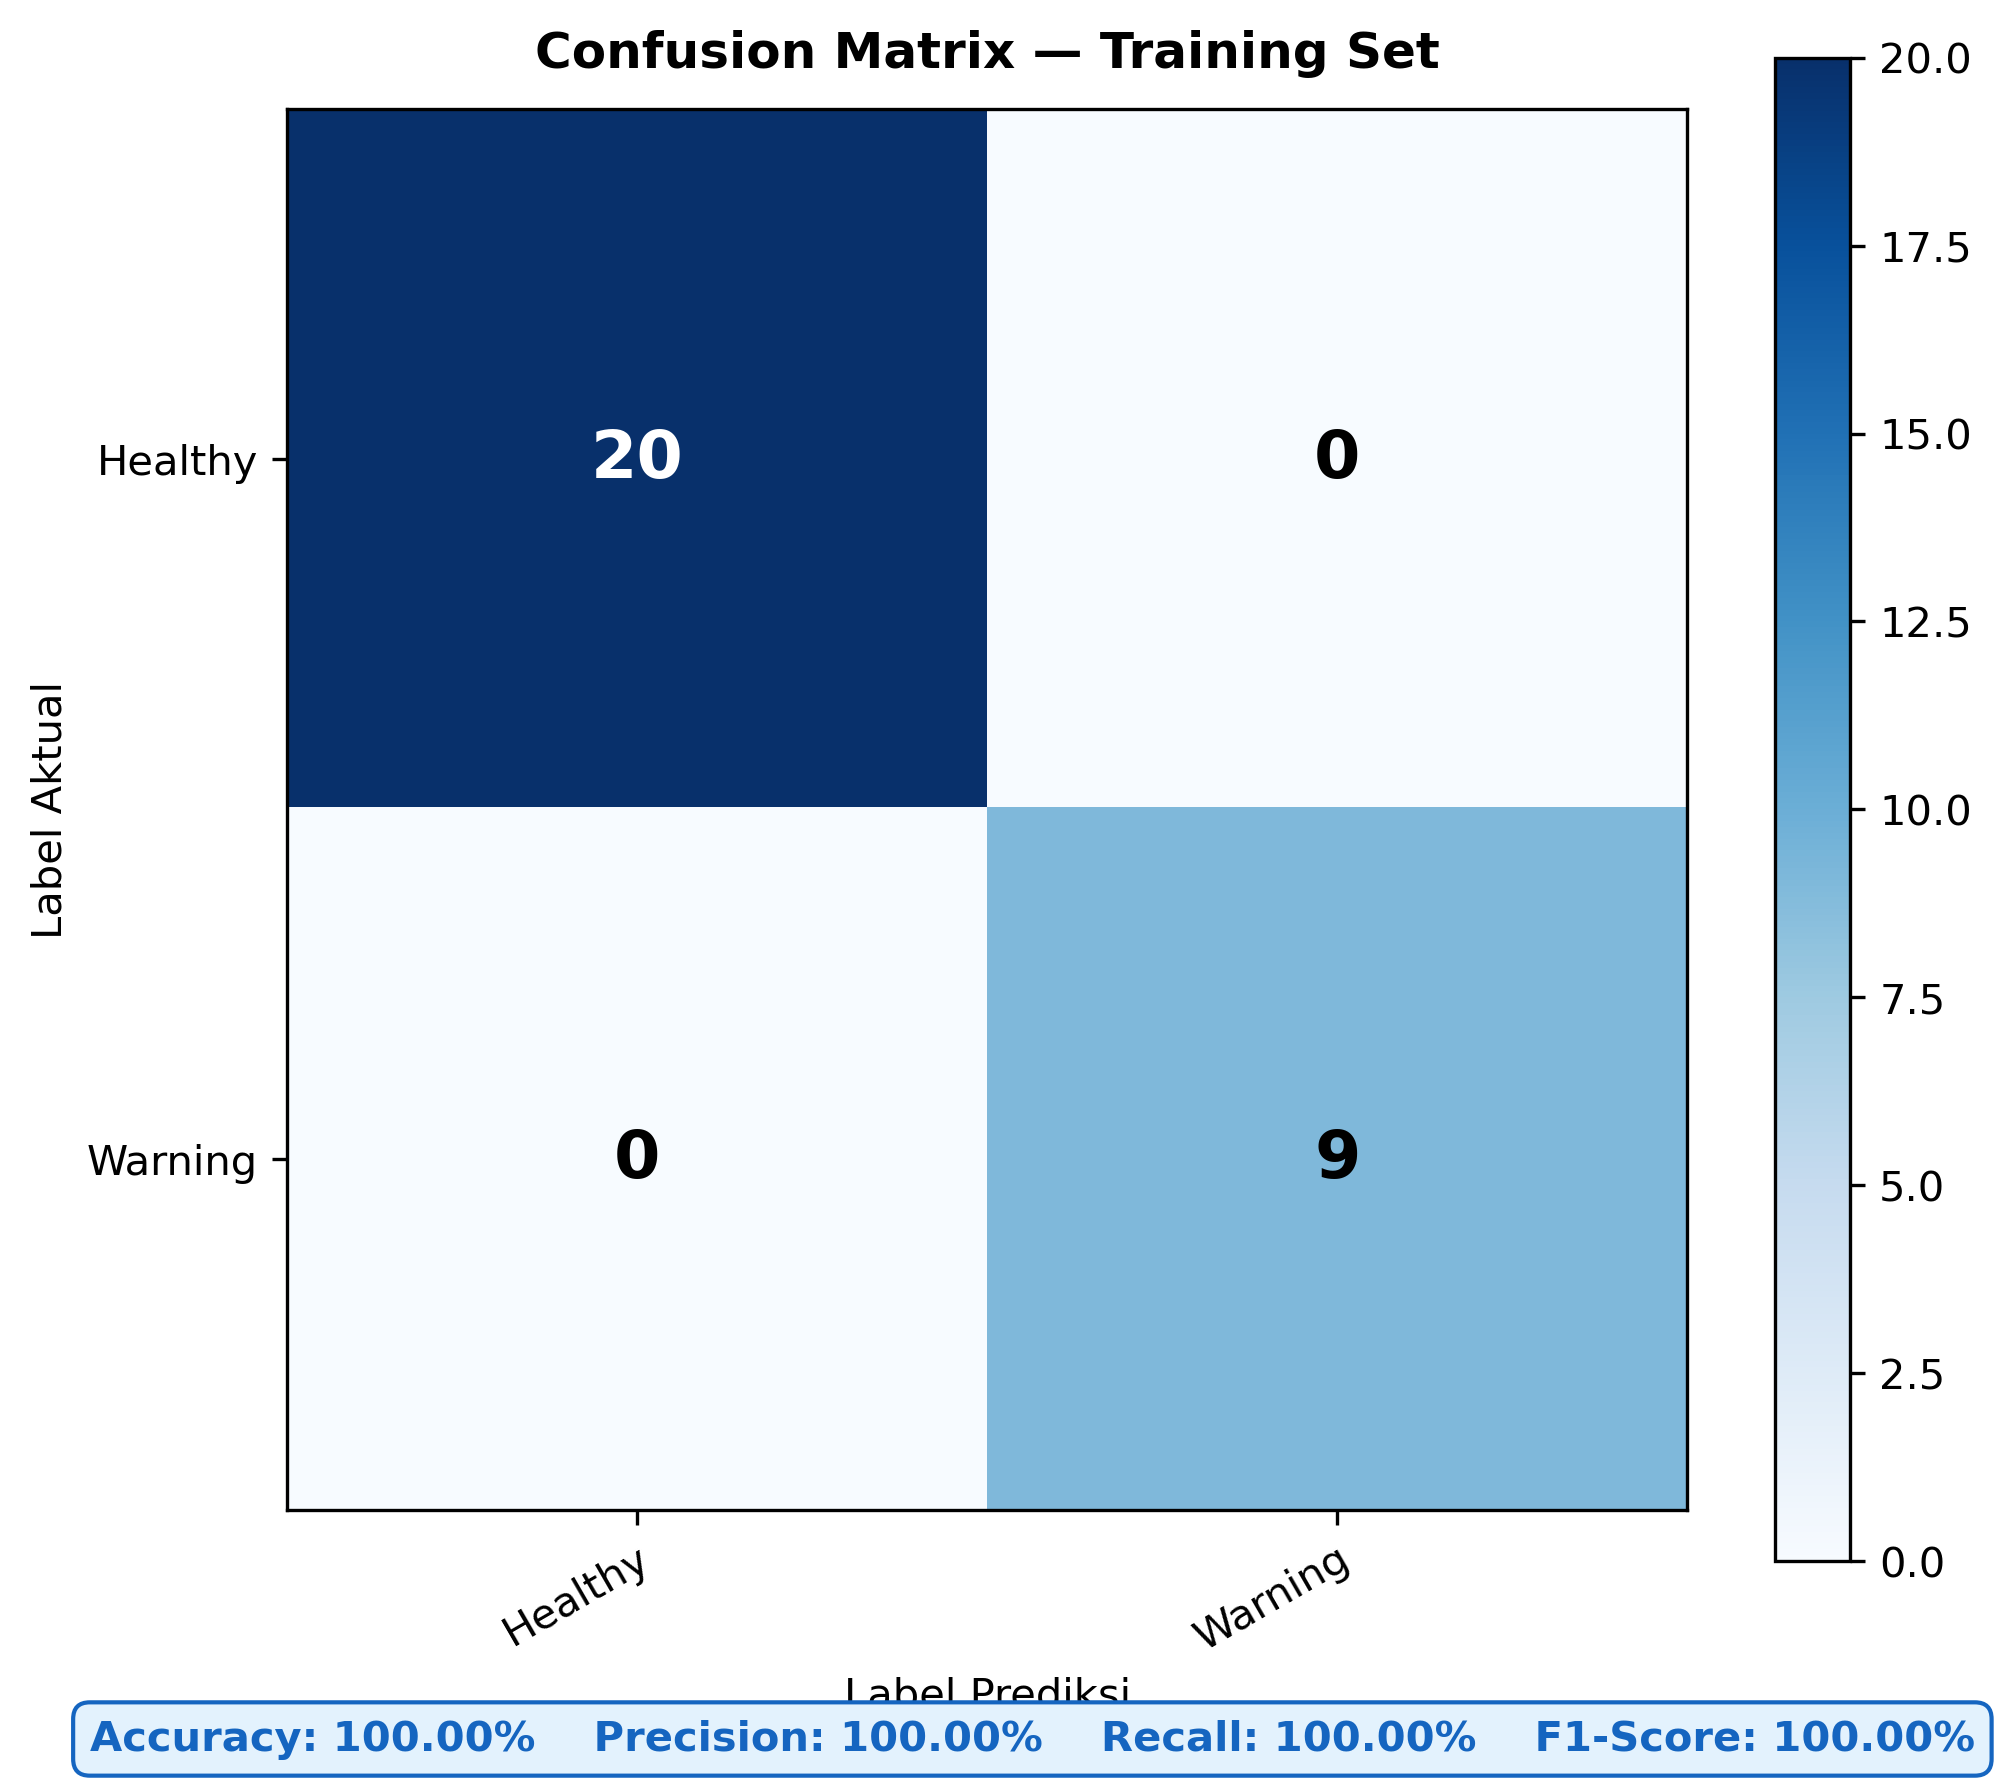
\includegraphics[width=0.75\linewidth]{jurnal_confusion_matrix_train.png}
    \caption{Confusion matrix Training Set — Acc=100,00\%, Prec=100,00\%, Rec=100,00\%, F1=100,00\%.}
    \label{fig:cmtrain}
\end{figure}

\begin{figure}[H]
    \centering
    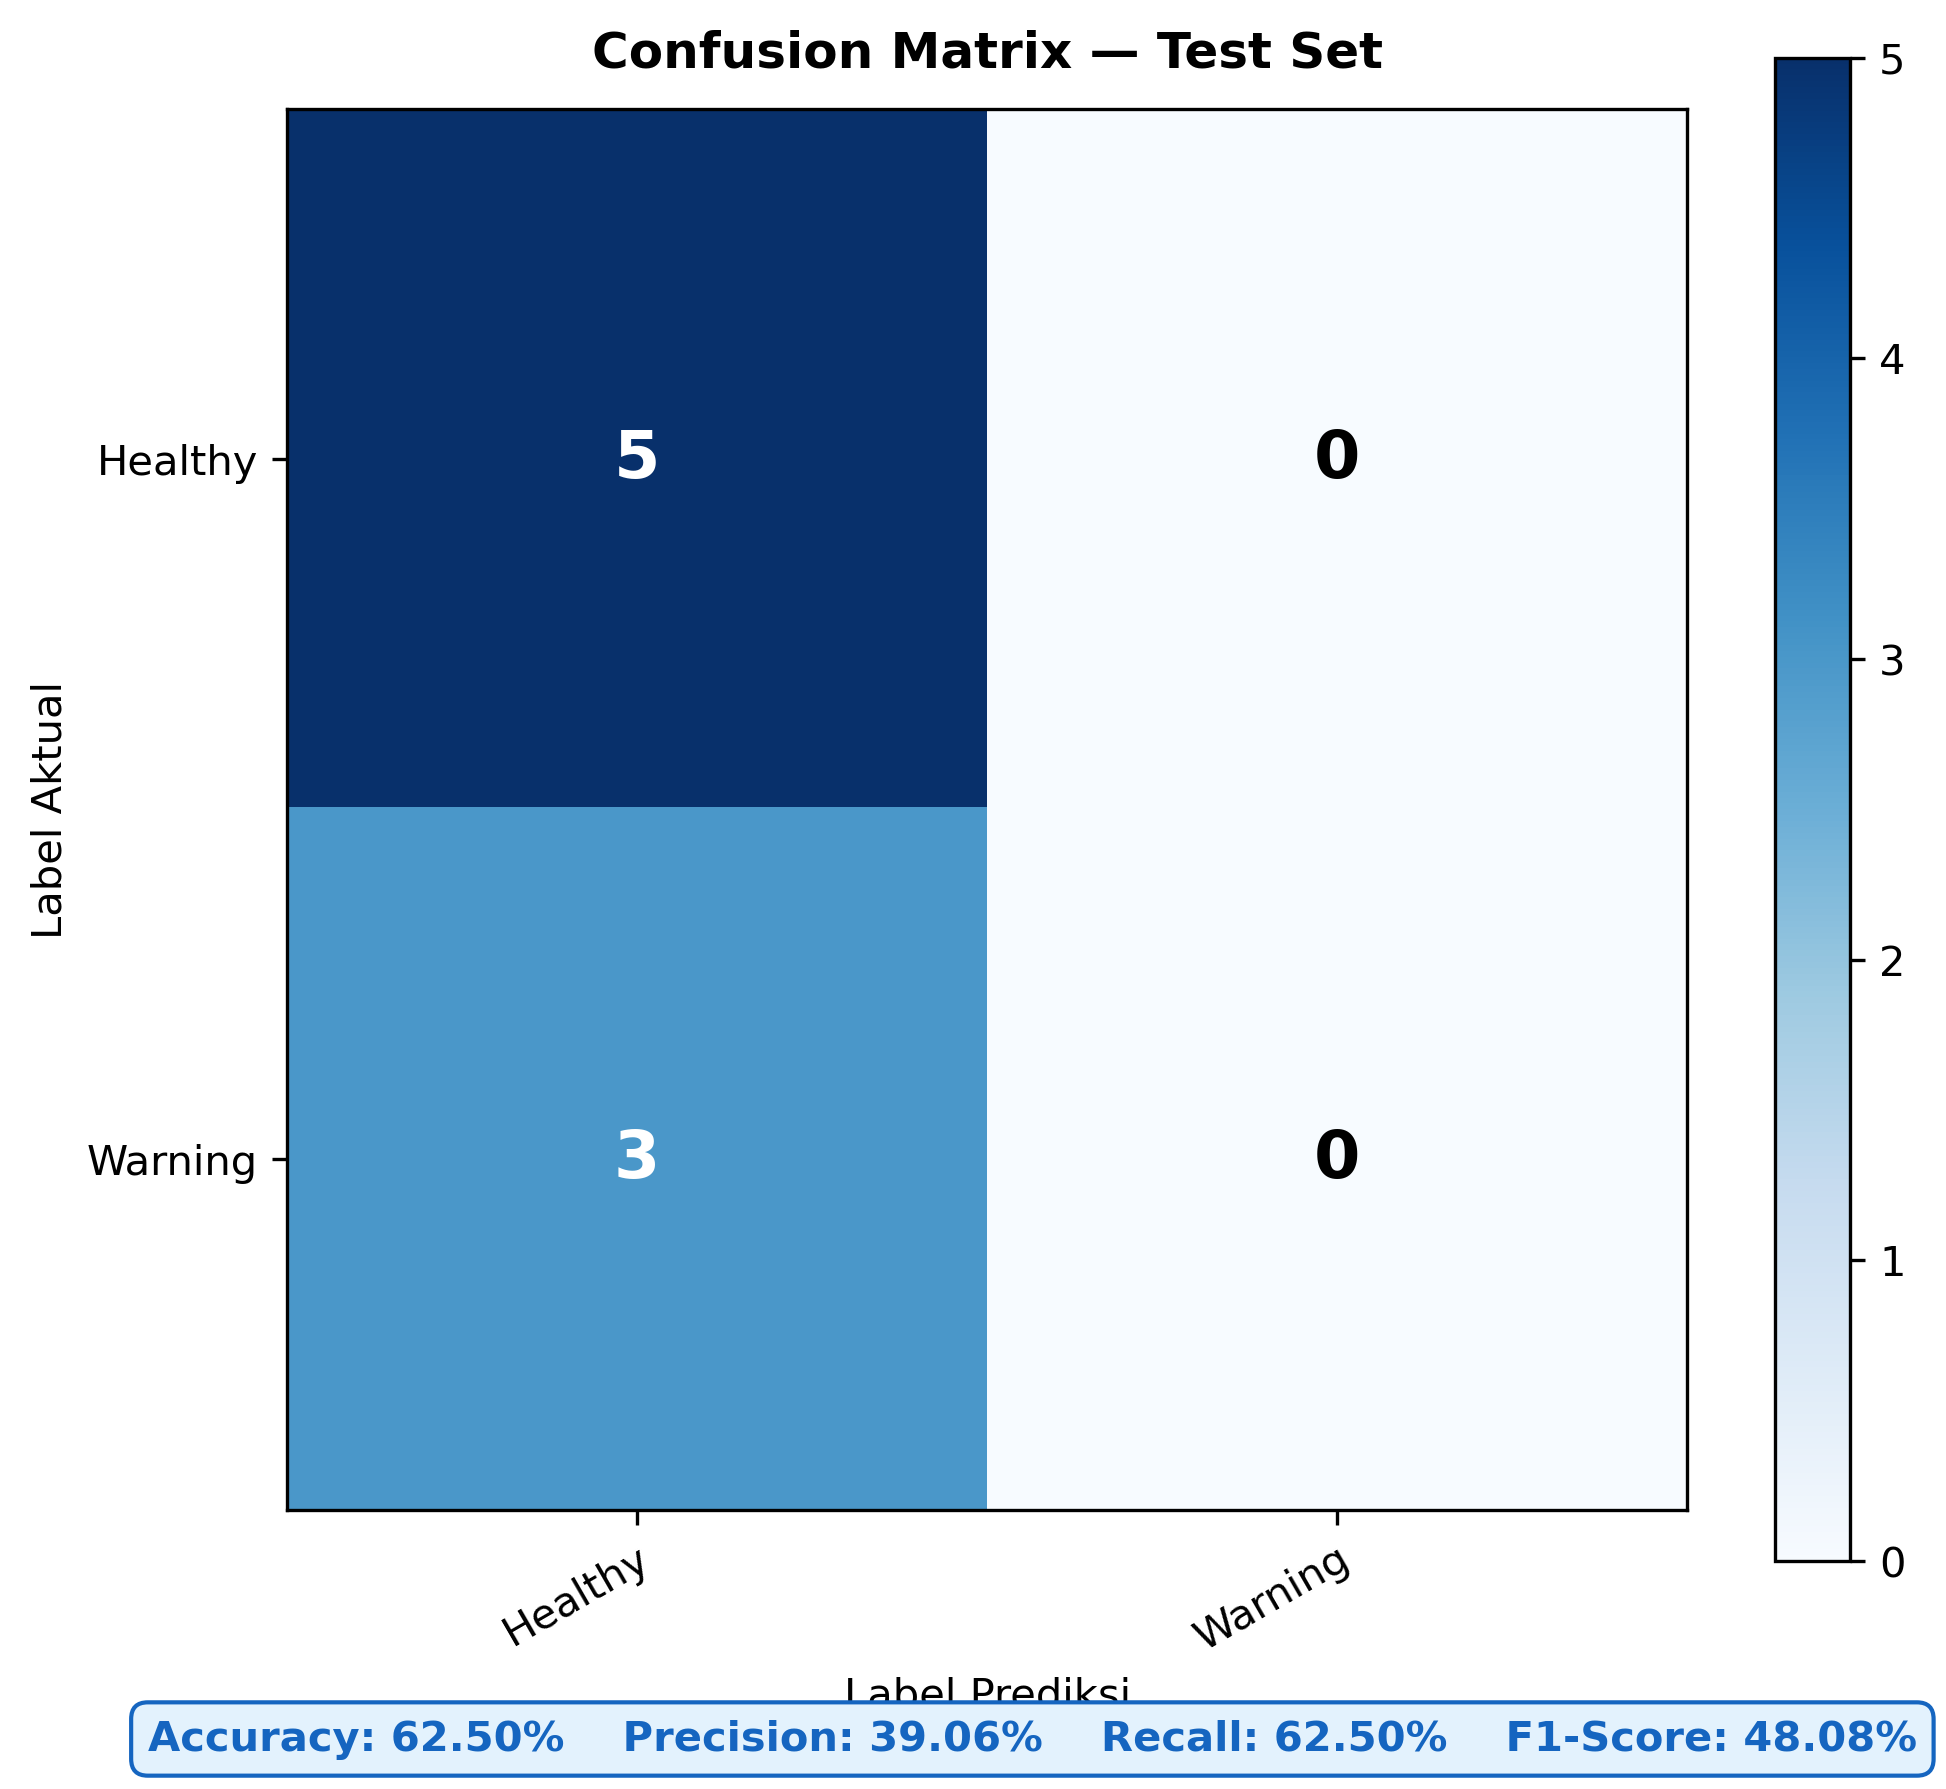
\includegraphics[width=0.75\linewidth]{jurnal_confusion_matrix_test.png}
    \caption{Confusion matrix Test Set — Acc=62,50\%, Prec=39,06\%, Rec=62,50\%, F1=48,08\%.}
    \label{fig:cmtest}
\end{figure}

\begin{table}[H]
    \centering
    \caption{Detail prediksi per hari — Test Set.}
    \begin{tabular}{clllc}
        \toprule
        \textbf{Day} & \textbf{Tanggal} & \textbf{Aktual} & \textbf{Prediksi} & \textbf{Benar?} \\
        \midrule
        30 & 09052026 & \healthy & \healthy & \ok \\
        31 & 14052026 & \warning & \healthy & \bad \\
        32 & 15052026 & \healthy & \healthy & \ok \\
        33 & 16052026 & \healthy & \healthy & \ok \\
        34 & 17052026 & \healthy & \healthy & \ok \\
        35 & 20052026 & \warning & \healthy & \bad \\
        36 & 22052026 & \warning & \healthy & \bad \\
        37 & 23052026 & \healthy & \healthy & \ok \\
        \bottomrule
    \end{tabular}
\end{table}

\begin{figure}[H]
    \centering
    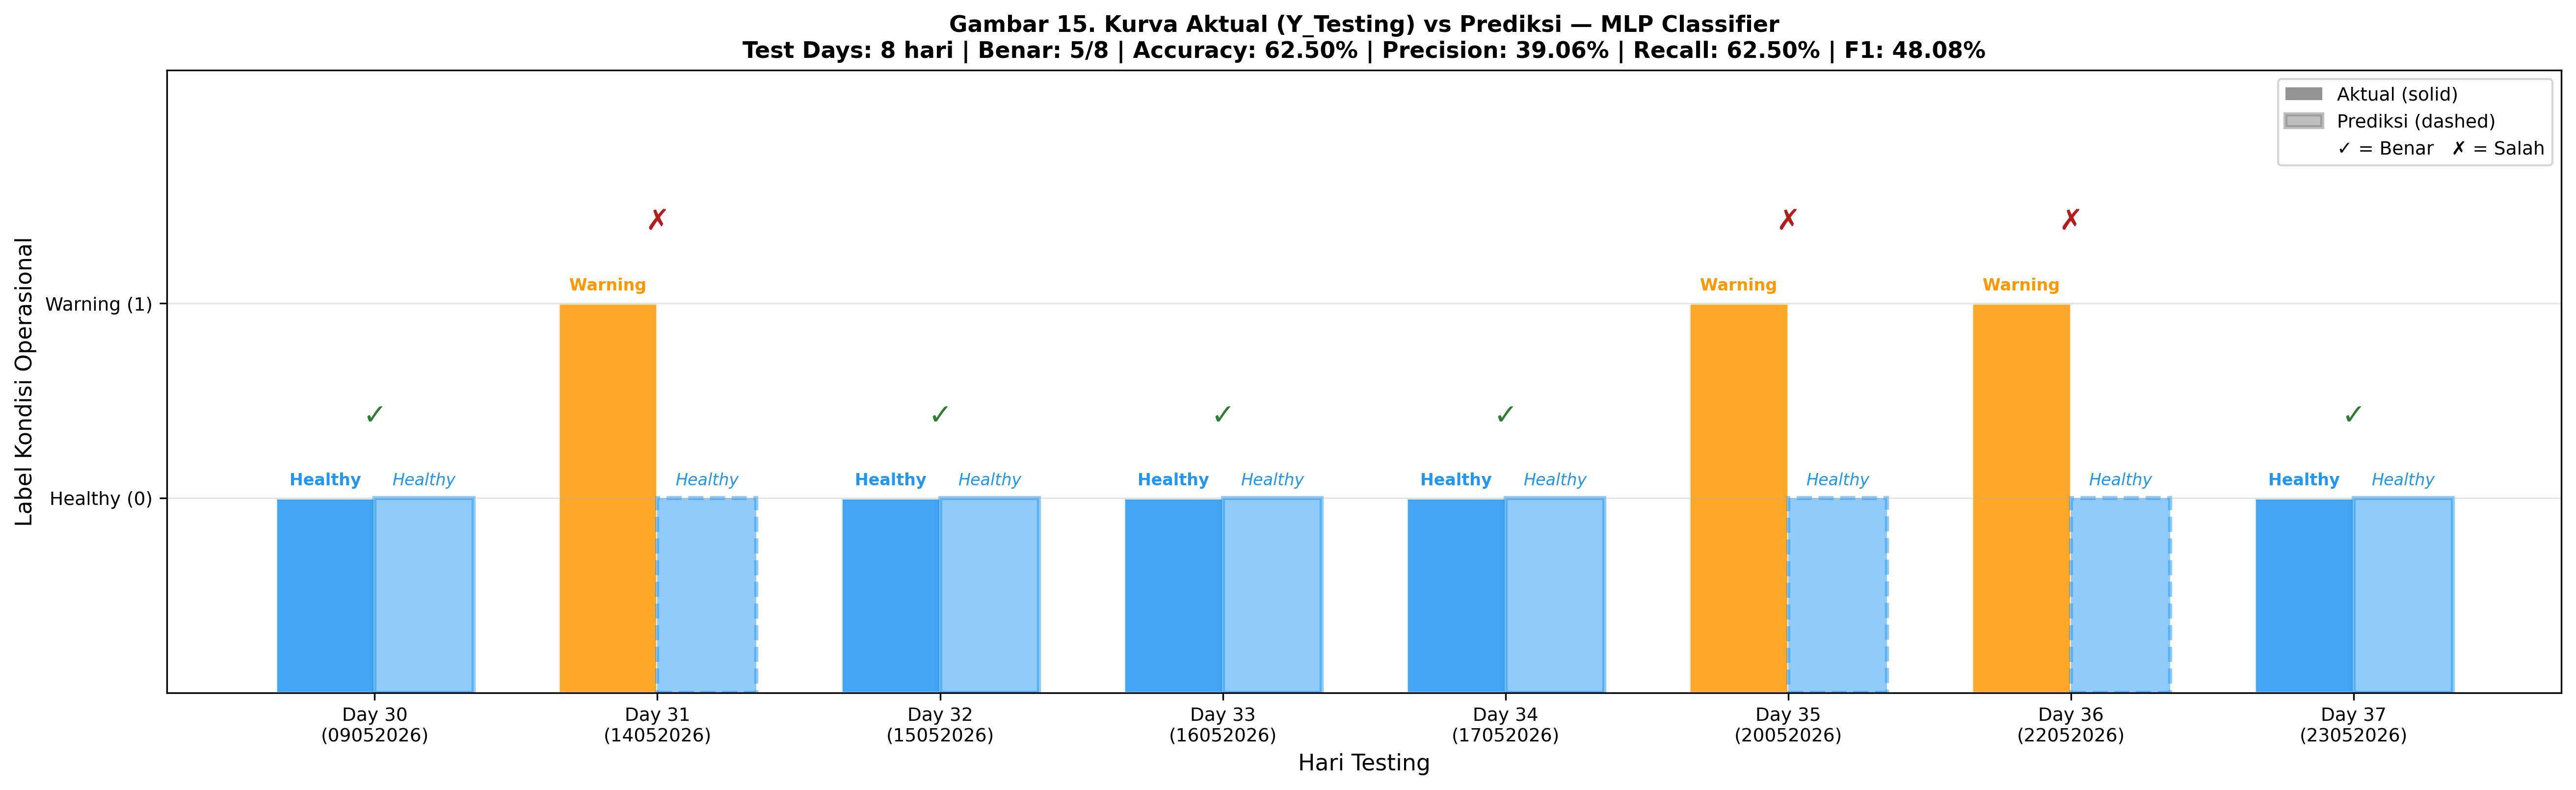
\includegraphics[width=0.8\linewidth]{jurnal_aktual_vs_prediksi_mlp.png}
    \caption{Perbandingan status aktual vs prediksi MLP Classifier per hari.}
    \label{fig:aktualpred}
\end{figure}

\subsection{Analisis Overfitting pada Stage 2}
Terdapat kesenjangan besar antara performa \textit{training} (Acc 100\%, CE 0,0002) dan \textit{testing} (Acc 62,5\%, CE 5,90). Model memprediksi \healthy\ untuk seluruh 8 hari \textit{test}, sehingga ketiga hari \warning\ aktual (Day 31, 35, 36) seluruhnya salah diklasifikasikan (\textit{recall} kelas Warning = 0\%). Penyebab yang diduga:
\begin{itemize}
    \item Ukuran dataset klasifikasi sangat kecil (29 sampel \textit{training}, hanya 9 sampel kelas Warning).
    \item Tidak ada mekanisme \textit{early stopping}; training berjalan penuh 100 epoch dengan \textit{learning rate} konstan.
    \item Model bias terhadap kelas mayoritas (Healthy) saat menghadapi data \textit{test} yang belum pernah dilihat.
\end{itemize}

\section{Inference}
\subsection{Training Inference (dengan Ground Truth)}
Tiga hari terakhir data \textit{training} digunakan untuk memprediksi hari pertama data \textit{testing}, sehingga \textit{ground truth} tersedia.

\begin{table}[H]
    \centering
    \caption{Detail Training Inference.}
    \begin{tabular}{ll}
        \toprule
        \textbf{Keterangan} & \textbf{Nilai} \\
        \midrule
        Input Hari A/B/C (Day 27--29) & 06052026 (Warning), 07052026 (Healthy), 08052026 (Healthy) \\
        Target Hari D (Day 30) & 09052026 \\
        Prediksi Status & \healthy\ (99,96\% confidence) \\
        Status Aktual & \healthy \\
        Klasifikasi & \ok\ BENAR \\
        MSE / RMSE / MAE & 0,004950 / 0,070358 / 0,037082 \\
        \bottomrule
    \end{tabular}
\end{table}

\begin{figure}[H]
    \centering
    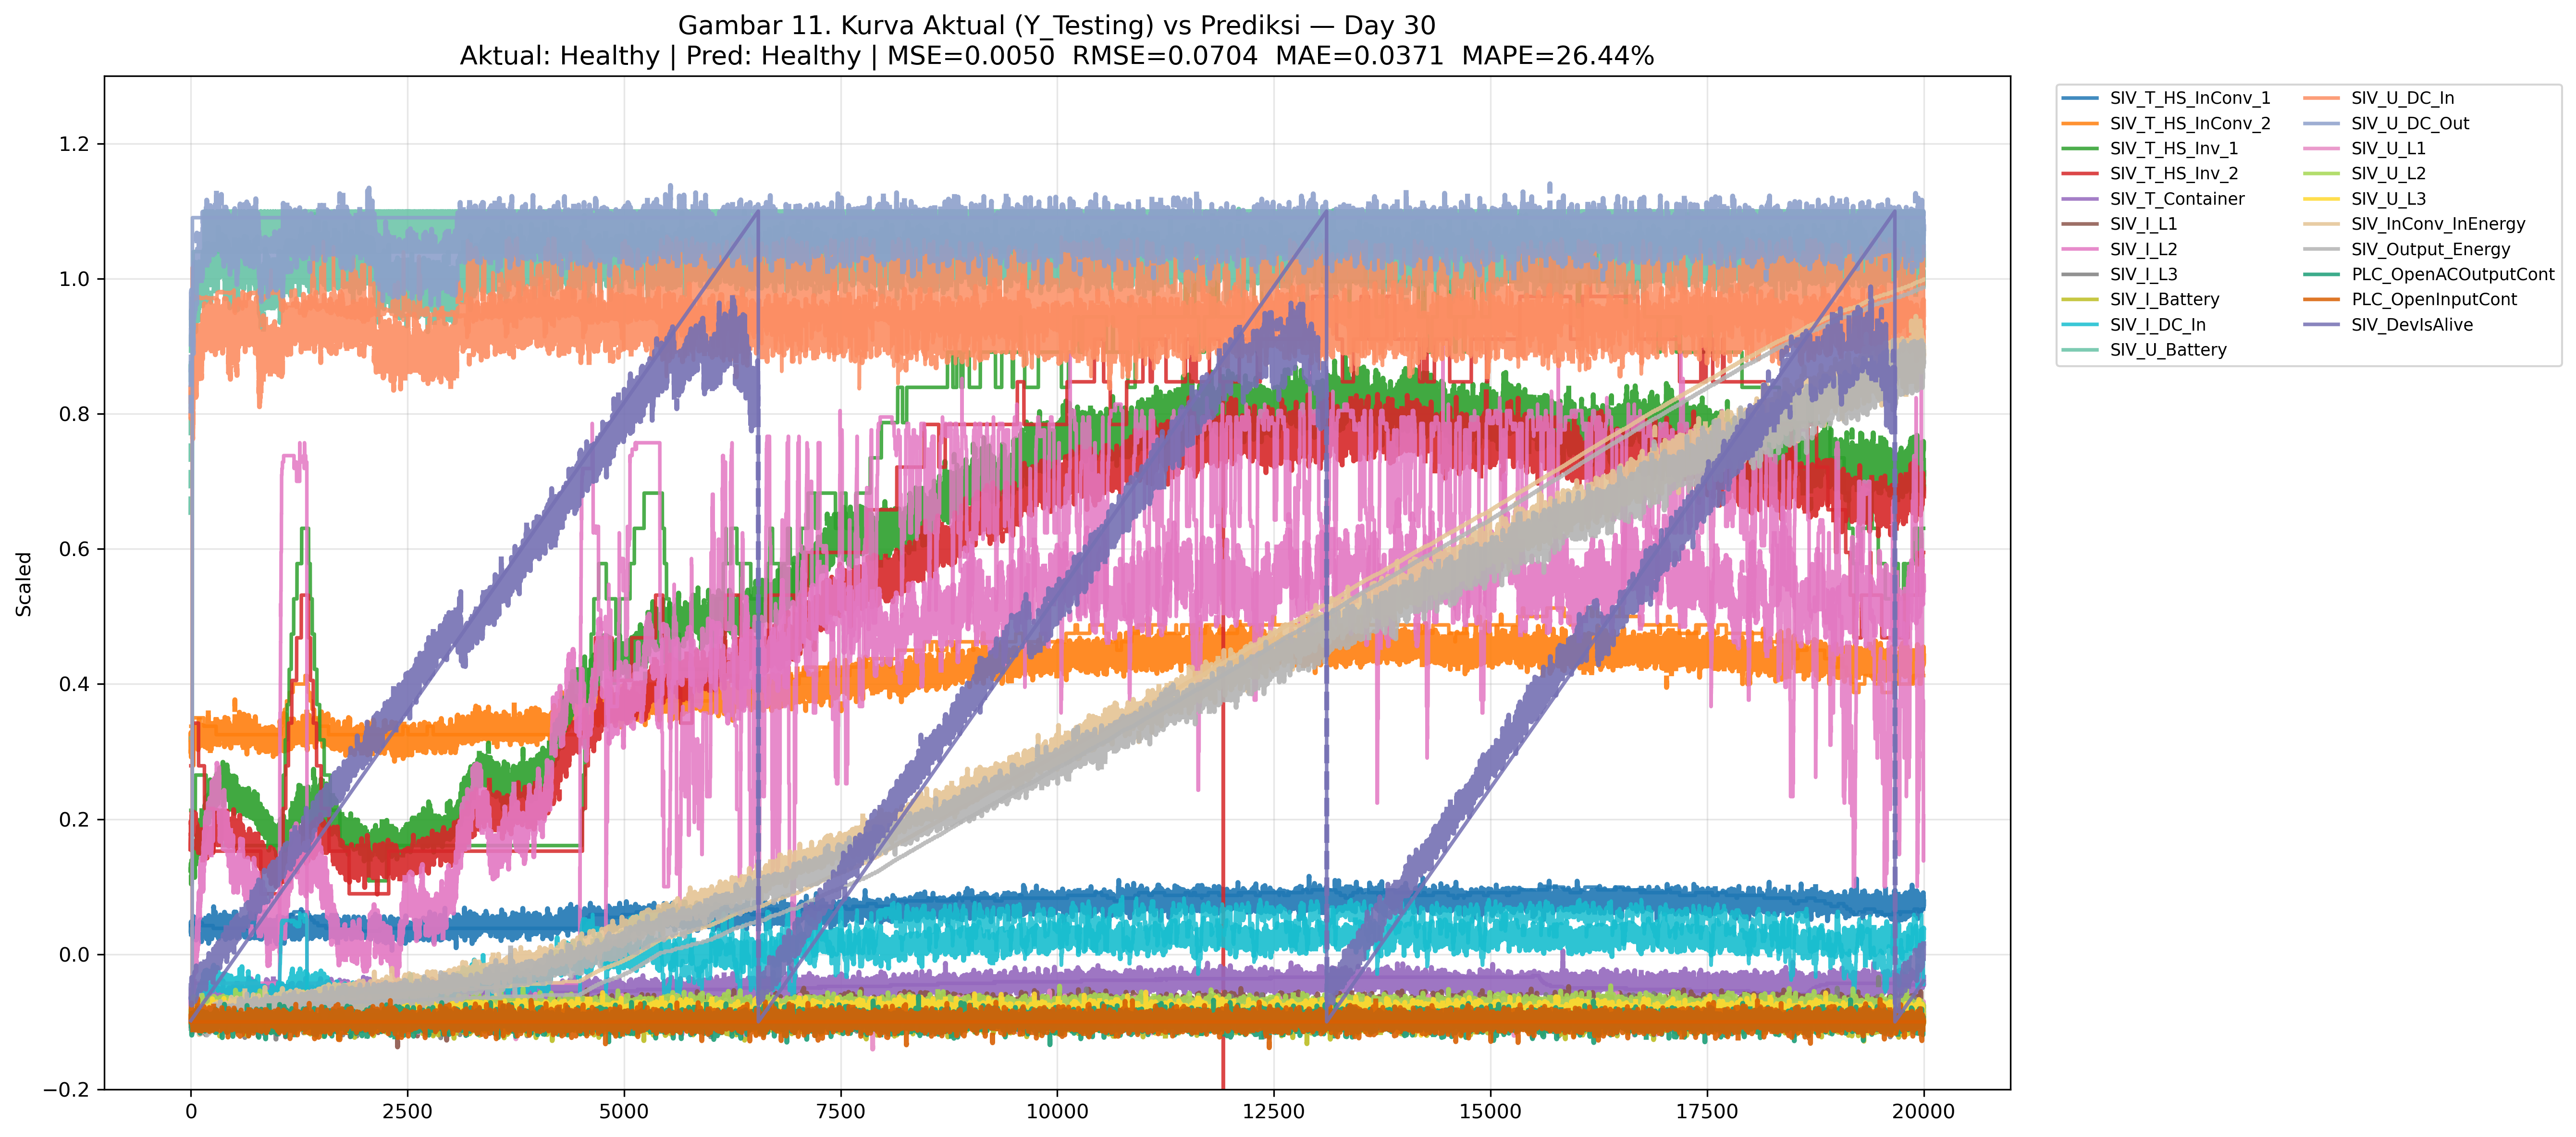
\includegraphics[width=0.8\linewidth]{gambar_train2_real_vs_pred.png}
    \caption{Training Inference — perbandingan aktual vs prediksi.}
    \label{fig:trainrealpred}
\end{figure}

\subsection{Testing Inference (tanpa Ground Truth)}
Tiga hari terakhir data \textit{testing} digunakan untuk memprediksi hari ke-38 (masa depan), sehingga tidak ada \textit{ground truth}.

\begin{table}[H]
    \centering
    \caption{Detail Testing Inference (forecasting masa depan).}
    \begin{tabular}{ll}
        \toprule
        \textbf{Keterangan} & \textbf{Nilai} \\
        \midrule
        Input Hari A/B/C (Day 35--37) & 20052026 (Warning), 22052026 (Warning), 23052026 (Healthy) \\
        Target & Hari ke-38 (masa depan) \\
        Prediksi Status & \healthy\ (99,96\% confidence) \\
        Ground Truth & Tidak tersedia \\
        \bottomrule
    \end{tabular}
\end{table}

\begin{figure}[H]
    \centering
    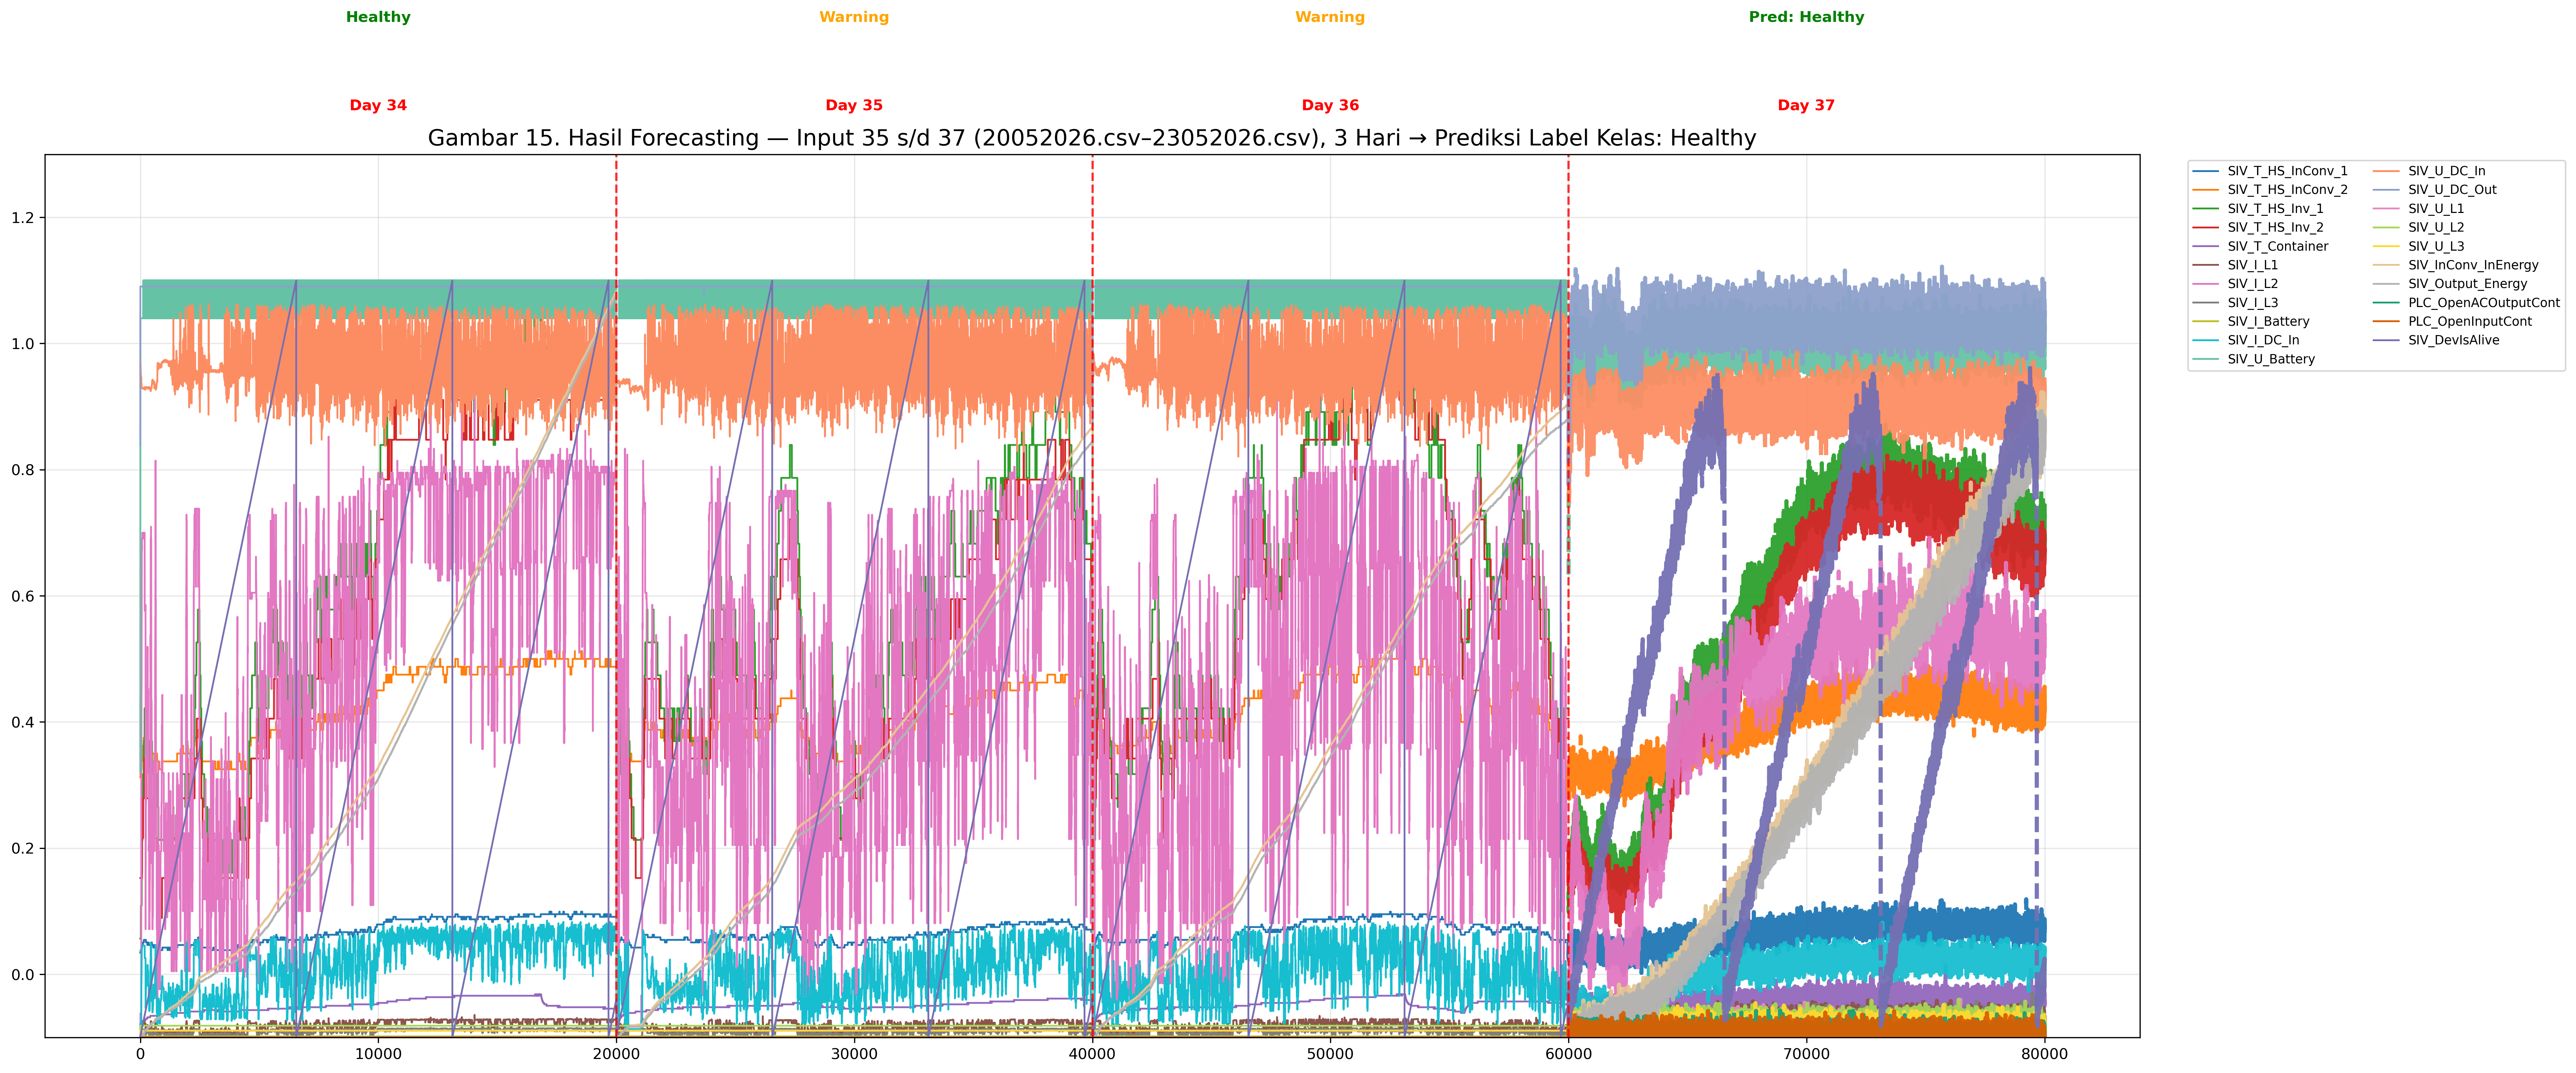
\includegraphics[width=0.8\linewidth]{gambar2_input_plus_prediksi_TCN.png}
    \caption{Testing Inference — hasil forecasting hari ke-38 beserta label kelas prediksi.}
    \label{fig:testforecast}
\end{figure}

\begin{table}[H]
    \centering
    \small
    \caption{Perbandingan Training Inference vs Testing Inference.}
    \begin{tabular}{lll}
        \toprule
        \textbf{Aspek} & \textbf{Training Inference} & \textbf{Testing Inference} \\
        \midrule
        Input Days & Day 27--29 (Train) & Day 35--37 (Test) \\
        Target & Day 30 (1st Test) & Day 38 (Future) \\
        Prediksi Status & \healthy\ (100,0\%) & \healthy\ (100,0\%) \\
        Ground Truth & \healthy & Tidak ada \\
        Klasifikasi Benar? & \ok\ BENAR & Tidak dapat diukur \\
        MSE/RMSE/MAE & 0,004950 / 0,070358 / 0,037082 & Tidak dapat diukur \\
        \bottomrule
    \end{tabular}
\end{table}

\section{Pembahasan Umum}
Hasil eksperimen menunjukkan bahwa tahap \textit{forecasting} (Stage 1 — TCN) memiliki performa yang stabil dan dapat digeneralisasi dengan baik, sedangkan tahap klasifikasi (Stage 2 — MLP) masih memerlukan perbaikan signifikan sebelum layak diterapkan pada kondisi operasional nyata, khususnya dalam mendeteksi kondisi \warning\ yang justru merupakan kelas paling krusial untuk sistem \textit{early warning}. Hal ini menegaskan pentingnya jumlah data berlabel yang memadai dalam membangun model klasifikasi berbasis \textit{deep learning}.

\newpage
% ============================================================
\chapter{KESIMPULAN DAN SARAN}
% ============================================================

\section{Kesimpulan}
\begin{enumerate}
    \item Model \textbf{TCN Forecaster (Stage 1)} berhasil memprediksi 21 parameter sensor SIV TS27 dengan performa baik dan stabil, ditunjukkan oleh selisih MSE \textit{train--test} yang kecil (MSE \textit{test} = 0,007446; RMSE = 0,086292; MAE = 0,043340).
    \item Model \textbf{MLP Classifier (Stage 2)} mencapai akurasi \textit{training} sempurna (100\%) namun mengalami penurunan signifikan pada data \textit{testing} (akurasi 62,5\%, F1-\textit{score} 48,08\%), mengindikasikan \textbf{overfitting} akibat keterbatasan jumlah data berlabel.
    \item Pendekatan dua tahap (TCN + MLP) secara konsisten memprediksi status \healthy\ pada inference \textit{training} (sesuai \textit{ground truth}) maupun inference masa depan, namun kemampuan model dalam mendeteksi kondisi \warning\ pada data \textit{testing} masih sangat terbatas.
    \item Secara keseluruhan, tahap \textit{forecasting} sinyal terbukti layak digunakan, sedangkan tahap klasifikasi kesehatan memerlukan penyempurnaan lebih lanjut sebelum dapat diandalkan sebagai sistem \textit{early warning} operasional.
\end{enumerate}

\section{Saran}
\begin{enumerate}
    \item \textbf{Penambahan data}: mengumpulkan lebih banyak hari berlabel, khususnya kelas \warning, untuk mengurangi \textit{class imbalance} dan meningkatkan kemampuan generalisasi model klasifikasi.
    \item \textbf{Early stopping}: menerapkan \textit{early stopping} berbasis \textit{validation loss} untuk mencegah \textit{overfitting} pada Stage 2.
    \item \textbf{Regularisasi tambahan}: mempertimbangkan peningkatan \textit{dropout}, \textit{weight decay}, atau pengurangan kapasitas model MLP.
    \item \textbf{Validasi silang}: menerapkan \textit{k-fold cross-validation} mengingat ukuran dataset yang terbatas, agar evaluasi performa lebih representatif.
    \item \textbf{Penelitian lanjutan}: mengeksplorasi arsitektur alternatif (misalnya LSTM, Transformer, atau pendekatan \textit{semi-supervised learning}) serta menguji model pada unit SIV lain untuk menguji generalisasi lintas unit.
\end{enumerate}

\newpage
% ============================================================
\chapter*{Daftar Pustaka}
\addcontentsline{toc}{chapter}{Daftar Pustaka}
% ============================================================
\noindent\textit{[Lengkapi daftar pustaka sesuai gaya sitasi yang diwajibkan institusi (APA/IEEE/dll). Contoh format IEEE:]}

\begin{enumerate}[label={[\arabic*]}]
    \item [Nama Penulis], "[Judul artikel]," \textit{[Nama Jurnal/Konferensi]}, vol. [x], no. [x], pp. [xx-xx], [Tahun].
    \item [Nama Penulis], \textit{[Judul Buku]}. [Kota]: [Penerbit], [Tahun].
\end{enumerate}

\newpage
% ============================================================
\chapter*{Lampiran}
\addcontentsline{toc}{chapter}{Lampiran}
% ============================================================
\begin{table}[H]
    \centering
    \small
    \caption{Daftar file data pendukung (folder \texttt{evidence/}).}
    \begin{tabular}{ll}
        \toprule
        \textbf{Nama File} & \textbf{Deskripsi} \\
        \midrule
        jurnal\_info\_stage1.txt & Hyperparameter, MSE train/test, tabel sequence \\
        jurnal\_info\_stage2.txt & Hyperparameter, CE/Acc, confusion matrix \\
        jurnal\_fitur\_statistik.csv & Mean/std/max/min per parameter per hari (84 kolom) \\
        inference\_train\_health\_status.csv & Hasil training inference \\
        inference\_health\_status.csv & Hasil testing inference \\
        model\_stage1\_forecaster.pth & Bobot model TCN terlatih \\
        model\_stage2\_classifier.pth & Bobot model MLP terlatih \\
        log\_stage1.txt / log\_stage2.txt & Log lengkap proses training \\
        \bottomrule
    \end{tabular}
\end{table}

\end{document}
